\documentclass[reprint,english,notitlepage]{revtex4-1}  % defines the basic parameters of the document

% if you want a single-column, remove reprint

% allows special characters (including æøå)
\usepackage[utf8]{inputenc}
\usepackage[english]{babel}

%% note that you may need to download some of these packages manually, it depends on your setup.
%% I recommend downloading TeXMaker, because it includes a large library of the most common packages.

\usepackage{physics,amssymb}  % mathematical symbols (physics imports amsmath)
\usepackage{graphicx}         % include graphics such as plots
\usepackage{xcolor}           % set colors
\usepackage{hyperref}         % automagic cross-referencing (this is GODLIKE)
\usepackage{tikz}             % draw figures manually
\usepackage{listings}         % display code
\usepackage{subfigure}        % imports a lot of cool and useful figure commands
\usepackage{cprotect}
\usepackage{float}


% defines the color of hyperref objects
% Blending two colors:  blue!80!black  =  80% blue and 20% black
\hypersetup{ % this is just my personal choice, feel free to change things
    colorlinks,
    linkcolor={red!50!black},
    citecolor={blue!50!black},
    urlcolor={blue!80!black}}

%% Defines the style of the programming listing
%% This is actually my personal template, go ahead and change stuff if you want
\lstnewenvironment{python}{
	\lstset{ %
		inputpath=,
		backgroundcolor=\color{white!88!black},
		basicstyle={\ttfamily\scriptsize},
		commentstyle=\color{magenta},
		language=Python,
		morekeywords={True,False},
		tabsize=4,
		stringstyle=\color{green!55!black},
		frame=single,
		keywordstyle=\color{blue},
		showstringspaces=false,
		columns=fullflexible,
		keepspaces=true}
}{}

\lstnewenvironment{cpp}{
	\lstset{ %
		inputpath=,
		backgroundcolor=\color{white!88!black},
		basicstyle={\ttfamily\scriptsize},
		commentstyle=\color{magenta},
		language=C++,
		morekeywords={True,False},
		tabsize=4,
		stringstyle=\color{green!55!black},
		frame=single,
		keywordstyle=\color{blue},
		showstringspaces=false,
		columns=fullflexible,
		keepspaces=true}
}{}

\lstset{literate=
  {á}{{\'a}}1 {é}{{\'e}}1 {í}{{\'i}}1 {ó}{{\'o}}1 {ú}{{\'u}}1
  {Á}{{\'A}}1 {É}{{\'E}}1 {Í}{{\'I}}1 {Ó}{{\'O}}1 {Ú}{{\'U}}1
  {à}{{\`a}}1 {è}{{\`e}}1 {ì}{{\`i}}1 {ò}{{\`o}}1 {ù}{{\`u}}1
  {À}{{\`A}}1 {È}{{\'E}}1 {Ì}{{\`I}}1 {Ò}{{\`O}}1 {Ù}{{\`U}}1
  {ä}{{\"a}}1 {ë}{{\"e}}1 {ï}{{\"i}}1 {ö}{{\"o}}1 {ü}{{\"u}}1
  {Ä}{{\"A}}1 {Ë}{{\"E}}1 {Ï}{{\"I}}1 {Ö}{{\"O}}1 {Ü}{{\"U}}1
  {â}{{\^a}}1 {ê}{{\^e}}1 {î}{{\^i}}1 {ô}{{\^o}}1 {û}{{\^u}}1
  {Â}{{\^A}}1 {Ê}{{\^E}}1 {Î}{{\^I}}1 {Ô}{{\^O}}1 {Û}{{\^U}}1
  {œ}{{\oe}}1 {Œ}{{\OE}}1 {æ}{{\ae}}1 {Æ}{{\AE}}1 {ß}{{\ss}}1
  {ű}{{\H{u}}}1 {Ű}{{\H{U}}}1 {ő}{{\H{o}}}1 {Ő}{{\H{O}}}1
  {ç}{{\c c}}1 {Ç}{{\c C}}1 {ø}{{\o}}1 {å}{{\r a}}1 {Å}{{\r A}}1
  {€}{{\euro}}1 {£}{{\pounds}}1 {«}{{\guillemotleft}}1
  {»}{{\guillemotright}}1 {ñ}{{\~n}}1 {Ñ}{{\~N}}1 {¿}{{?`}}1
}



\usepackage{thmtools}
\DeclareMathOperator{\nullspace}{Nul}
\DeclareMathOperator{\collspace}{Col}
\DeclareMathOperator{\rref}{Rref}
%%\DeclareMathOperator{\dim}{Dim}

 % "meq": must be equal
\newcommand{\meq}{\overset{!}{=}}
\newcommand\numberthis{\addtocounter{equation}{1}\tag{\theequation}}

\newcommand{\R}{\mathbb{R}}
\newcommand*\Heq{\ensuremath{\overset{\kern2pt L'H}{=}}}
\usepackage{bm}
\newcommand{\uveci}{{\bm{\hat{\textnormal{\bfseries\i}}}}}
\newcommand{\uvecj}{{\bm{\hat{\textnormal{\bfseries\j}}}}}
\DeclareRobustCommand{\uvec}[1]{{%
  \ifcsname uvec#1\endcsname
     \csname uvec#1\endcsname
   \else
    \bm{\hat{\mathbf{#1}}}%
   \fi
}}
\usepackage[binary-units=true]{siunitx}

\makeatletter
\newcommand*{\balancecolsandclearpage}{%
  \close@column@grid
  \cleardoublepage
  \twocolumngrid
}
\makeatother

\newcounter{subproject}
\renewcommand{\thesubproject}{\alph{subproject}}
\newenvironment{subproj}{
\begin{description}
	\item[\refstepcounter{subproject}(\thesubproject)]
}{\end{description}}


\begin{document}
\title{Project 3}   % self-explanatory
\author{Eivind Støland, Anders P. Åsbø}               % self-explanatory
\date{\today}                             % self-explanatory
\noaffiliation                            % ignore this

\maketitle                                % creates the title, author, date


\tableofcontents

\section{Introduction} \label{sec:I}
Differential equations are the mathematical description of continuous change, and thus one of the most important cornerstones of physics since their invention. In spite of how often they appear in physics, few differential equations have analytic solutions, and as such it is vital to be able to approximate a solution numerically.

In this report, we will derive two different methods of numerical integration, namely the forward Euler method and the velocity Verlet method. To test important properties of the methods, such as conservation of energy, conservation of angular momentum and numerical stability, we will apply the methods to solve the differential equations that arise in celestial mechanics when simulating the motion of objects in our Solar System.

We firstly apply both methods to solve the Sun-Earth two-body system with only gravitational interaction. The simulations are performed with varying precision to ascertain the stability and convergence of each method.

Furthermore, we use the velocity Verlet method to simulate orbits of an Earth-like object with initial velocity close to the Sun’s escape velocity at a \(1\) AU distance. We also simulate the Sun-Earth system for both circular and non-circular orbits, using variations of Newtonian gravity that are not pure inverse-square laws. To test our implementation's ability to solve a system with no analytic solution, we apply the velocity Verlet method to simulate a \(3\)-body system consisting of the Sun, Earth and Jupiter, with different masses for Jupiter per simulation.

To test the generality of our implementation, we apply the velocity Verlet method to simulate an \(n\)-body system consisting of the Sun with eight planets and Pluto.

Finally, we apply the velocity Verlet method together with a relativistic correction of Newton's law of gravitation to simulate the perihelion precession of Mercury's orbit. A simulation with no relativistic correction is also done for comparison.

\section{Formalism} \label{sec:II}

\subsection{Two methods for numerical integration} \label{sec:II:a}
To solve our equations of motion we require methods for numerical integration. To derive our first method, we consider the generic function \(f\) that depends on a variable \(t\) such that
\begin{align*}
	\frac{d}{dt}f(t) = g(t, f(t)). \numberthis \label{eq:fofg}
\end{align*}
Given an arbitrary point \(f(t_{0})\), we wish to approximate the point \(f(t_{1})\). Thus we can integrate each side of \eqref{eq:fofg}, such that
\begin{align*}
	\int_{t_{0}}^{t_{1}} \frac{d}{dt} f(t) dt = \int_{t_{0}}^{t_{1}} g(t, f(t)) dt.
\end{align*}
Applying the fundemental theorem of calculus, we get that
\begin{align*}
	f(t_{1}) - f(t_{0}) = \int_{t_{0}}^{t_{1}} g(t, f(t)) dt, \\
	f(t_{1}) = f(t_{0}) + \int_{t_{0}}^{t_{1}} g(t, f(t)) dt. \numberthis \label{eq:foft1}
\end{align*}
To complete the approximation, we define a step-length \(\Delta t = t_{1}-t_{0}\), and approximate the area under the curve of \(g(t, f(t))\) between \(g(t_{0}, f(t_{0})\) and \(g(t_{1}, f(t_{1}))\) as the area of a rectangle whith height \(g(t_{0}, f(t_{0}))\). Inserting the rectangle approximation into \eqref{eq:foft1} yields
\begin{align*}
	f(t_{0} + \Delta t) \approx f(t_{0}) + \Delta t g(t_{0}, f(t_{0})).
\end{align*}

As we neglect all terms of second order or higher in this approximation we have that the error goes as $\mathcal{O}(\Delta t^2)$. 
If we want to approximate a value \(f(t_{k+1})\), we can simply start with a known value at a \(t_{k} < t_{k+1}\) and take a step with our approximation such that
\begin{align*}
	f(t_{k+1}) \approx f(t_{k}) + \Delta t g(t_{k}, f(t_{k})).
\end{align*}
Finally we can simplify the notation by setting \(f_{k+1} = f(t_{k})\) resulting in
\begin{align*}
	f_{k+1} = f_{k} + \Delta t g(t_{k}, f_{k}). \numberthis \label{eq:forwardEuler}
\end{align*}
This method of numerical integration is known as Euler's method, henceforth referred to as the forward Euler method.

Since we are approximating the integral between each pair of \(g(t, f_{k})\) and \(g(t, f_{k+1})\)  as a single rectangle with width \(\Delta t\), our approximation will be more accurate for smaller values of \(\Delta t\). Thus to approximate the curve of the function \(f\), we create a set of \(f_{k}\) values for a given \(f_{0}\) and \(\Delta t\) by repeatedly taking steps using the forward Euler method.

Many physical problems can be represented by a second order differential equation:

\begin{align*}
\frac{d^2}{dt^2} \vec{x}(t) &= \vec{a}(t,\vec{x}(t)) \, , \numberthis \label{eq:sodiff}
\end{align*}

where $\vec{x}(t)$ is the function we want to find and $\vec{a}(t,\vec{x}(t))$ is a function dependent on $\vec{x}(t)$. As the parts of this equation are vectors, this is actually a set of $D$ differential equations, where $D$ is the length of the vectors. This differential equation can be split into $2D$ first order differential equations:

\begin{align*}
\frac{d}{dt} \vec{v}(t) &= \vec{a}(t,\vec{x}(t))  \\
\frac{d}{dt} \vec{x}(t) &= \vec{v}(t) \, , \numberthis \label{eq:sodiff_split}
\end{align*}

When split into first order differential equations like this we can easily solve this system using methods such as the forward Euler method given a set of initial conditions. 

%In this kind of system we can make a small adaptation to the forward Euler method. The method with this small change is called the Euler-Cromer method (using the same discretization that was described earlier): 

%\begin{align*}
%\vec{v}_{k+1} &= \vec{v}_k + \Delta t  \vec{a}(t_k, \vec{x}_k) \\
%\vec{x}_{k+1} &= \vec{x}_k + \Delta t \vec{v}_{k+1} \numberthis \label{eq:EulerCromer}
%\end{align*}  

%Instead of using $\vec{v}_k$ to calculate $\vec{x}_{k+1}$ we use the next step $\vec{v}_{k+1}$. This improves the accuracy of the numerical solution. 

Another method used to solve the system of equations in \eqref{eq:sodiff_split} is the velocity Verlet algorithm. We will now derive this algorithm. First we Taylor expand $\vec{x}(t + \Delta t)$:

\begin{align*}
\vec{x}(t + \Delta t) &= \vec{x}(t) + \Delta t \vec{v}(t) + \frac{\Delta t^2}{2} \vec{a}(t) + \mathcal{O}(\Delta t^3) \numberthis \label{eq:so_taylorx}
\end{align*}

Using the discretization described earlier, along with defining $\vec{x}(t_k) = \vec{x}_k$ and $\vec{v}(t_k) = \vec{v}_k$ we can rewrite this equation: 

\begin{align*}
\vec{x}_{k + 1} &\approx \vec{x}_k + \Delta t \vec{v}_k + \frac{\Delta t^2}{2} \vec{a}(t_k,\vec{x}_k) \numberthis \label{eq:so_taylorx_disc}
\end{align*}

Similarly we can also Taylor expand $\vec{v}(t+\Delta t)$:

\begin{align*}
\vec{v}(t+\Delta t) &= \vec{v}(t) + \Delta t \vec{a}(t) + \frac{\Delta t^2}{2} \frac{d}{dt} \vec{a}(t) + \mathcal{O}(\Delta t^3) \numberthis \label{eq:so_taylorv}
\end{align*}

We do not know what $\frac{d}{dt} \vec{a}(t)$ is, but we can approximate it:

\begin{align*}
\frac{d}{dt}\vec{a}(t) &= \frac{\vec{a}(t+\Delta t) - \vec{a}(t)}{\Delta t} + \mathcal{O}(\Delta t^2) \\
\Delta t \frac{d}{dt} \vec{a}(t) &= \vec{a}(t+ \Delta t ) - \vec{a}(t) + \mathcal{O}(\Delta t^3) 
\end{align*}

Inserting this into \eqref{eq:so_taylorv} gives:

\begin{align*}
\vec{v}(t+\Delta t) &= \vec{v}(t) + \Delta t \vec{a}(t) + \frac{\Delta t}{2} (\vec{a}(t+ \Delta t ) - \vec{a}(t)) + \mathcal{O}(\Delta t^3) \\
&= \vec{v}(t) + \frac{\Delta t}{2} (\vec{a}(t+ \Delta t ) + \vec{a}(t)) +  \mathcal{O}(\Delta t^3) 
\end{align*}

Discretizing this gives:

\begin{align*}
\vec{v}_{k+1} &\approx \vec{v}_k + \frac{\Delta t}{2} \bigg( \vec{a}(t_{k+1}, \vec{x}_{k+1}) + \vec{a}(t_k, \vec{x}_k) \bigg)
\end{align*}

Combining this with \eqref{eq:so_taylorx_disc} gives us the velocity Verlet algorithm:

\begin{align*}
\vec{x}_{k+1} &= \vec{x}_k + \Delta t \vec{v}_k + \frac{1}{2} \Delta t^2 \vec{a}(t_k,\vec{x}_k) \\
\vec{v}_{k+1} &= \vec{v}_k + \frac{1}{2}\Delta t \bigg( \vec{a}(t_{k+1},x_{k+1}) + \vec{a}(t_k, \vec{x}_k) \bigg) \, . \numberthis \label{eq:VelocityVerlet}
\end{align*}

In this algorithm we first move the position one step, and then use this when calculating $\vec{v}$ in the next step. This algorithm has two advantages over the forward Euler method. Firstly it is approximately symplectic, meaning that if it is used to solve a set of equations given by Newton's second law there is little to no energy drift. Secondly the error of the approximation goes as $\mathcal{O}(\Delta t^3)$ compared to $\mathcal{O}(\Delta t^2)$ for the forward Euler method.

\subsection{A generalized gravitational force} \label{sec:II:b}
For any two bodies \(a\) and \(b\), the gravitational force acting on body \(a\) from body \(b\) is
\begin{align*}
	\vec{F}_{a} = -G\frac{m_{a}m_{b}}{|\vec{r}_{a}-\vec{r}_{b}|^{3}}\left(\vec{r}_{a}-\vec{r}_{b}\right), \numberthis \label{eq:grav} \\
\end{align*}
where \(m_{a}\) and \(m_{b}\) are the masses of \(a\) and \(b\) respectivly, \(\vec{r}_{a}\) and \(\vec{r}_{b}\) are the position vectors of \(a\) and \(b\) respectivly, and \(G\) is the gravitational constant. The potential energy and the force are connected by the relation $\vec{F} = - \gradient U$. This gives us that the potential energy has to be:

\begin{align*}
U &= - G \frac{m_a m_b}{|\vec{r}_a - \vec{r}_b|} \numberthis \label{eq:pot_en}
\end{align*}

For a circular motion of body $a$ around $b$ this should remain constant as the distance between the objects is always the same. The total energy in such a two-body system is also conserved, and this means that the kinetic energy also has to be conserved, as the total energy is the sum of the kinetic and potential energy. At this point this is just an assumption, but we will prove it in the next section. In an elliptical motion however, only the total energy is conserved, and we will see oscillations in the kinetic and potential energy.

If we consider a body in a \(n\)-body system where the only interaction is gravitational, the net force on any body \(i\) becomes the sum of all the forces on body \(i\) from every other body in the system. Using \eqref{eq:grav} and summing over all bodies \(j\), where \(j\neq i\), we get
\begin{align*}
	\vec{F}_{i} = -Gm_{i}\sum_{j\neq i}m_{j}\frac{\vec{r}_{i}-\vec{r}_{j}}{|\vec{r}_{i}-\vec{r}_{j}|^{3}}. \numberthis \label{eq:gengrav}
\end{align*}

We then find the acceleration of body \(i\) at time \(t\) by dividing the net force by \(m_{a}\) resulting in
\begin{align*}
	\vec{a}_{i}(t) = \frac{\vec{F}_{i}(t)}{m_{i}} = -G\sum_{j\neq i}m_{j}\frac{\vec{r}_{i}(t)-\vec{r}_{j}(t)}{|\vec{r}_{i}(t)-\vec{r}_{j}(t)|^{3}}, \numberthis \label{eq:accel}
\end{align*}
which can be written as the differential equation
\begin{align*}
 	\frac{d\vec{v}_{i}(t)}{dt} = -G\sum_{j\neq i}m_{j}\frac{\vec{r}_{i}(t)-\vec{r}_{j}(t)}{|\vec{r}_{i}(t)-\vec{r}_{j}(t)|^{3}}. \numberthis \label{eq:gendv}
\end{align*}
In addition we have the differential equation
\begin{align*}
	\frac{d\vec{r}_{i}(t)}{dt} = \vec{v}(t) \numberthis \label{eq:gendr}.
\end{align*}

Solving \eqref{eq:gendv} and \eqref{eq:gendr} for every body \(i=1, ..., n\), allows us to find the internal motion of a given n-body system with only gravitational interaction. In this system we can also define total potential energy:

\begin{align*}
U_\text{tot} &= \sum\limits_i - G m_i \sum\limits_{j\neq i} \frac{m_j}{|\vec{r}_i - \vec{r}_j|} \, , \numberthis \label{eq:tot_pot_en}
\end{align*}

and the total kinetic energy:

\begin{align*}
K_\text{tot} &= \sum\limits_i \frac{1}{2}m_i \vec{v}_i^2 \numberthis \label{eq:tot_kin_en}
\end{align*}

The sum of the total kinetic and potential energy of the system should be constant (this will be proven in the next section). This can be used to test the algorithms.

We will also be experimenting with a slightly different form of the force in \eqref{eq:grav}:

\begin{align*}
\vec{F}_a = - G \frac{m_a m_b}{|\vec{r}_a - \vec{r}_b|^{\beta + 1} } ( \vec{r}_a - \vec{r}_b) \, , \numberthis \label{eq:beta_grav}
\end{align*}

where $\beta \in [2,3]$ is a real constant. Choosing $\beta = 2$ corresponds to the normal gravitational force, and choosing a $\beta$ larger than this means that the force will be stronger for objects that are closer to each other and weaker for those that are far from each other. In a $n$-body system such as in \eqref{eq:gengrav} we have that the total force an object experiences is:

\begin{align*}
\vec{F}_{i} = -Gm_{i}\sum_{j\neq i}m_{j}\frac{\vec{r}_{i}-\vec{r}_{j}}{|\vec{r}_{i}-\vec{r}_{j}|^{\beta + 1}}. \numberthis \label{eq:beta_gengrav}
\end{align*}

We can also write down the total potential energy in this case:

\begin{align*}
U_\text{tot} &= \sum\limits_i - \frac{G m_i}{\beta - 1} \sum\limits_{j\neq i} \frac{m_j}{|\vec{r}_i - \vec{r}_j|^{\beta-1}} . \numberthis \label{eq:beta_tot_pot_en}
\end{align*}

The total kinetic energy remains the same in this case.

\subsection{Conservation of energy} \label{sec:II:c}

We have that the force $\vec{F}$ is related to the potential energy as follows:

\begin{align*}
\vec{F} &= - \gradient U \numberthis \label{eq:force_pot_en}
\end{align*}

This will be useful later. That the total energy $E$ is conserved can be written mathematically as:

\begin{align*}
\frac{dE}{dt} &= 0 \\
\frac{d}{dt} (K_\text{tot} + U_\text{tot}) &= 0 \, ,
\end{align*} 

where we have used that the total energy is the sum of the total kinetic energy $K_\text{tot}$ and the total potential energy $U_\text{tot}$. We now assume that we are in an $n$-body system, where the potential energy is velocity independent. The potential energy is determined by the interaction between the bodies and a potential time dependent part. We define $\vec{r}_{ij} = \vec{r}_i - \vec{r}_j$ as the distance vector between the position of body $i$ ($\vec{r}_i$) and body $j$ ($\vec{r}_j$). This means that we can write the total potential energy as:

\begin{align*}
U_\text{tot} = \frac{1}{2}\sum\limits_i \sum\limits_{j\neq i} U(\vec{r}_{ij},t) \, ,
\end{align*}

where $U$ here is the potential energy experienced by body $i$ because of body $j$. The factor $1/2$ comes from the fact that we cannot sum up the potential energy between two objects twice. This also means that we can write the force experienced by body $i$ from body $j$ as:

\begin{align*}
\vec{F}_{ij} = - \gradient_{ij} U(\vec{r}_{ij}, t) \, ,
\end{align*}

where $\gradient_{ij}$ differentiates with respect to $\vec{r}_{ij}$. We can then write the time derivative of the potential energy as:

\begin{align*}
\frac{d}{dt}U_\text{tot} &= \frac{1}{2}\sum\limits_{i} \sum\limits_{j\neq i} \frac{d}{dt} U (\vec{r}_{ij}, t ) \, , \\
&= \frac{1}{2}\sum\limits_{i} \sum\limits_{j\neq i} \bigg( \gradient_{ij} U (\vec{r}_{ij}, t ) \cdot \frac{d\vec{r}_{ij}}{dt} + \frac{\partial }{\partial t} U(\vec{r}_{ij}, t) \bigg) \\
&= \frac{\partial}{\partial t} U_\text{tot} + \frac{1}{2}\sum\limits_{i} \sum\limits_{j\neq i} \gradient_{ij} U (\vec{r}_{ij}, t ) \cdot \frac{d\vec{r}_{ij}}{dt} \\
&= \frac{\partial}{\partial t} U_\text{tot} - \frac{1}{2}\sum\limits_{i} \sum\limits_{j\neq i} \vec{F}_{ij} \cdot \frac{d\vec{r}_{ij}}{dt} \numberthis \label{eq:pot_en_der}
\end{align*}

The total kinetic energy can be given as the sum of the kinetic energy of each body:

\begin{align*}
K_\text{tot} &= \sum\limits_i \frac{1}{2} m \vec{v}_i^2 
\end{align*}

The time derivative of this is:

\begin{align*}
\frac{d}{dt} K_\text{tot} &= \sum\limits_i m \vec{v}_i \cdot \vec{a}_i \\
&= \sum\limits_i \frac{d\vec{r}_i}{dt} \cdot \vec{F}_i \\
&= \frac{1}{2}\sum\limits_i \sum\limits_{i\neq j} \frac{d\vec{r}_i}{dt} \cdot \vec{F}_{ij} - \frac{1}{2}\sum\limits_i \sum\limits_{i\neq j} \frac{d\vec{r}_j}{dt} \cdot \vec{F}_{ij} \\
&= \frac{1}{2}\sum\limits_i \sum\limits_{i\neq j} \frac{d\vec{r}_{ij}}{dt} \cdot \vec{F}_{ij} \numberthis \label{eq:kin_en_der1}
\end{align*}


where $\vec{F}_i$ is the total force body $i$ experiences given as $\vec{F}_i = \sum\limits_{j\neq i} \vec{F}_{ij}$ as long as there are no external forces. The second to last equality is non-trivial, which means we need to prove it. We have that:

\begin{align*}
\sum\limits_i \frac{d\vec{r}_i}{dt} \cdot \vec{F}_i &= \sum\limits_i \sum\limits_{j \neq i} \frac{d\vec{r}_i}{dt} \cdot \vec{F}_{ij} 
\end{align*}

We can also recognize by using Newton's third law ($\vec{F}_{ij} = - \vec{F}_{ji}$) that:

\begin{align*}
\sum\limits_i \sum\limits_{j \neq i} \frac{d\vec{r}_i}{dt} \cdot \vec{F}_{ij} &= -\sum\limits_i \sum\limits_{j \neq i} \frac{d\vec{r}_i}{dt} \cdot \vec{F}_{ji} 
\end{align*}

By changing the index labels on the right-hand side we get:

\begin{align*}
\sum\limits_i \sum\limits_{j \neq i} \frac{d\vec{r}_i}{dt} \cdot \vec{F}_{ij} &= -\sum\limits_j \sum\limits_{i \neq j} \frac{d\vec{r}_j}{dt} \cdot \vec{F}_{ij} 
\end{align*}

As the intention of the double summation is to sum over every combination of $i$ and $j$ where $i\neq j$ it is arbitrary in which order we sum over the variables, as long as the inequality is kept as part of the inner sum:

\begin{align*}
\sum\limits_i \sum\limits_{j \neq i} \frac{d\vec{r}_i}{dt} \cdot \vec{F}_{ij} &= -\sum\limits_i \sum\limits_{j \neq i} \frac{d\vec{r}_j}{dt} \cdot \vec{F}_{ij} 
\end{align*}

Putting this all together, we can write:

\begin{align*}
\sum\limits_i \frac{d\vec{r}_i}{dt} \cdot \vec{F}_i &= \sum\limits_i \sum\limits_{j \neq i} \frac{d\vec{r}_i}{dt} \cdot \vec{F}_{ij} \\
&= \frac{1}{2} \sum\limits_i \sum\limits_{j \neq i} \frac{d\vec{r}_i}{dt} \cdot \vec{F}_{ij} + \frac{1}{2} \sum\limits_i \sum\limits_{j \neq i} \frac{d\vec{r}_i}{dt} \cdot \vec{F}_{ij} \\
&= \frac{1}{2} \sum\limits_i \sum\limits_{j \neq i} \frac{d\vec{r}_i}{dt} \cdot \vec{F}_{ij} - \frac{1}{2} \sum\limits_i \sum\limits_{j \neq i} \frac{d\vec{r}_j}{dt} \cdot \vec{F}_{ij} \, , \numberthis \label{eq:pos_force_dot_sum}
\end{align*}

which is the relation we wanted to show. Our requirement for the energy to be conserved was that:

\begin{align*}
\frac{d}{dt}(K_\text{tot} + U_\text{tot}) &= 0
\end{align*}

Using \eqref{eq:pot_en_der} and \eqref{eq:kin_en_der1} in this gives us:

\begin{align*}
\frac{1}{2}\sum\limits_i \sum\limits_{i\neq j} \frac{d\vec{r}_{ij}}{dt} \cdot \vec{F}_{ij} + \frac{\partial}{\partial t} U_\text{tot} - \frac{1}{2}\sum\limits_{i} \sum\limits_{j\neq i} \vec{F}_{ij} \cdot \frac{d\vec{r}_{ij}}{dt} &= 0 \\
\frac{\partial}{\partial t} U_\text{tot} &= 0 \\
\frac{1}{2}\sum\limits_i \sum\limits_{j\neq i } \frac{\partial}{\partial t} U(\vec{r}_{ij},t) &= 0 \numberthis \label{eq:energy_cons}
\end{align*}

In other words for an $n$-body system to have conserved energy we need the potential energy to be independent of time. Another assumption made along the way was that there are no external forces, which means that this is only for a closed system. This proves that total energy is conserved both in $n$-body systems where the force interaction is given by \eqref{eq:gengrav} or \eqref{eq:beta_gengrav} as there are no external forces and the potential energies (\eqref{eq:tot_pot_en} and \eqref{eq:beta_tot_pot_en} respectively) are time independent.


\subsection{Conservation of angular momentum} \label{sec:II:d}

Kepler's second law states that the position vector between a planet and the Sun sweeps out a constant area for a given interval of time, no matter the starting position of the planet in its orbit. Mathematically this can be formulated as follows:

\begin{align*}
\frac{dA}{dt} &= \frac{r^2}{2} \frac{d\theta}{dt} \, , \numberthis \label{eq:kepler_second}
\end{align*}   

where $A$ is the area swept by the position vector, $r$ is the length of the position vector and $\theta$ is the angle determining the direction of the position vector. It is implicit here that we are looking at the 2D plane that the planet orbits the Sun in as the $xy$-plane, as this simplifies the equation significantly. 

The angular momentum is given by:

\begin{align*}
\ell &= |\vec{r} \cross \vec{p}| \, ,\numberthis \label{eq:ang_mom}
\end{align*}

where $\vec{r}$ is the position vector, and $\vec{p} = m \vec{v}$ is the momentum vector with $\vec{v}$ being the velocity vector and $m$ being the mass. Now we can make some assumptions. Assuming that the position vector rotates in the $xy$-plane the only contribution to the cross product comes from the tangential component of the velocity $v_\theta$. If we assume the tangential velocity to be in positive $\theta$-direction (we can always transform the chosen plane so that this is the case) we get:

\begin{align*}
\ell &= mrv_\theta \numberthis \label{eq:2D_ang_mom}
\end{align*}

Using that $\vec{v} = \frac{d}{dt} \vec{r}$ we can write:

\begin{align*}
v_\theta &= r \frac{d\theta}{dt}
\end{align*}

We can insert this along with \eqref{eq:2D_ang_mom} into \eqref{eq:kepler_second}:

\begin{align*}
\frac{dA}{dt} &= \frac{r^2}{2} \frac{d\theta}{dt} \\
\frac{dA}{dt} &= \frac{r}{2} v_\theta \\
\frac{dA}{dt} &= \frac{1}{2} \frac{\ell}{m} 
\end{align*}

Since we already know that the left-hand side of this equation is constant this directly implies that the size of the angular momentum is a conserved quantity as we also assume the mass to be constant. 

For a system of $n$-bodies such as in the previous sections we can define the total angular momentum of a system as:

\begin{align*}
\vec{L}_\text{tot} &= \sum\limits_i \vec{r}_i \cross m\vec{v}_i \numberthis \label{eq:tot_ang_mom}
\end{align*}

This quantity should be conserved as long as there are no external forces, and the forces are conservative. We can prove that this is the case for both the forces we use in this report (\eqref{eq:gengrav} and \eqref{eq:beta_gengrav}). That the angular momentum is conserved means that:

\begin{align*}
\frac{d}{dt} \vec{L} &= 0 \, , 
\end{align*}

where 0 here corresponds to the zero vector technically. We find that the left-hand side of this can be written as:

\begin{align*}
\frac{d}{dt} \vec{L} &= \frac{d}{dt} (\sum\limits_i \vec{r}_i \cross m \vec{v}_i)  \\
&= \sum\limits_i \vec{v}_i \cross m \vec{v}_i + \vec{r}_i \cross m \vec{a}_i \\
&= \sum\limits_i \vec{r}_i \cross \vec{F}_i  \, , \numberthis \label{eq:interm_ang_mom_cons}
\end{align*}

where $\vec{F}_i$ is the force on body $i$, $\vec{a}_i$ is the acceleration on body $i$ and all other quantities are as previously defined. The cross product of a vector with itself is the zero vector, so that is why the $\vec{v} \cross \vec{v}$ term disappeared. Now we can use a result similar to the one found in \eqref{eq:pos_force_dot_sum}:

\begin{align*}
\sum\limits_i \vec{r}_i \cross \vec{F}_i &= \sum\limits_i \sum\limits_{j \neq i} \vec{r}_i \cross \vec{F}_{ij} \\
&= \frac{1}{2} \sum\limits_i \sum\limits_{j \neq i} \vec{r}_i \cross \vec{F}_{ij} + \frac{1}{2} \sum\limits_i \sum\limits_{j \neq i} \vec{r}_i \cross \vec{F}_{ij} \\
&= \frac{1}{2} \sum\limits_i \sum\limits_{j \neq i} \vec{r}_i \cross \vec{F}_{ij} - \frac{1}{2} \sum\limits_i \sum\limits_{j \neq i} \vec{r}_j \cross \vec{F}_{ij} \\
&= \frac{1}{2} \sum\limits_i \sum\limits_{j\neq i } \vec{r}_{ij} \cross \vec{F}_{ij} \, , \numberthis \label{eq:pos_cross_force_sum}
\end{align*}

where $\vec{r}_{ij}$ is the distance vector between body $i$ and $j$. In both the forces we use in this report (\eqref{eq:gengrav} and \eqref{eq:beta_gengrav}) the force is in the direction of $\vec{r}_{ij}$. This means we can write $\vec{F}_{ij} = f_{ij} \vec{r}_{ij}$ where $f_{ij}$ is a scalar. Using this along with \eqref{eq:pos_cross_force_sum} in \eqref{eq:interm_ang_mom_cons} gives:

\begin{align*}
\frac{d}{dt} \vec{L} &= \sum\limits_i \vec{r}_i \cross \vec{F}_i \\
&= \frac{1}{2} \sum\limits_i \sum\limits_{j\neq i } \vec{r}_{ij} \cross \vec{F}_{ij} \\
&= \frac{1}{2} \sum\limits_i \sum\limits_{j\neq i } \vec{r}_{ij} \cross f_{ij} \vec{r}_{ij} \\
&= 0 \, , \numberthis \label{eq:ang_mom_cons}
\end{align*}

where we again used that the cross-product of a vector with itself is the zero-vector. This shows that the angular momentum is conserved.

\subsection{Escape velocity of object in gravitational field} \label{sec:II:e}

An object has a velocity large enough to escape a gravitational field when the total energy of the object is larger than zero. In other words we need the velocity $v$ to fulfill the following requirement:

\begin{align*}
K + U &\geq 0 \\
\frac{1}{2}mv^2 - \frac{GMm}{r} &\geq 0 \\
v &\geq \sqrt{\frac{2GM}{r}} \, ,
\end{align*}

where $K$ is the kinetic energy, $U$ the potential energy, $G$ the gravitational constant, $m$ the mass of the object, $M$ the mass of the object causing the gravitational field, $r$ the distance between them, and $v$ the size of the velocity of the object relative to the object causing the field. The escape velocity $v_e$ is the lowest velocity that allows escape in this way, and is thus given by the formula:

\begin{align*}
v_e &= \sqrt{\frac{2GM}{r}} \numberthis \label{eq:esc_vel}
\end{align*}

If we consider a planet at a distance of \(1\) AU from the Sun, we can calculate its escape velocity as
\begin{align*}
	v_{sun, 1} = \sqrt{\frac{2\cdot 4\pi^{2}\cdot 1}{1}} \text{ AU/year},
\end{align*}
using the Sun's mass as our unit mass, and \(G = 4\pi^{2}\). Thus we get
\begin{align*}
	v_{sun, 1} = 2\pi\sqrt{2}\text{ AU/year}, \numberthis \label{eq:esc_sun_1au}
\end{align*}
as the escape velocity of a planet starting at a distance of \(1\) AU from the Sun.

\subsection{Perihelion precession of Mercury} \label{sec:II:f}

The observed precession of Mercury's perihelion is about 43'' per century when all contributions from classical effects are subtracted. By adding a relativistic correction term we can verify that we obtain the same result. The gravitational force between Mercury and the Sun with the relativistic correction term is as follows:

\begin{align*}
F_G &= \frac{GM_\text{Mercury} M_\text{Sun}}{r^2} \bigg[ 1 + \frac{3l^2}{r^2 c^2}\bigg] \, , \numberthis \label{eq:grav_rel} 
\end{align*}

where $M_\text{Mercury}$ is the mass of Mercury, $M_\text{Sun}$ the mass of the Sun, $r$ the distance between Mercury and the Sun, $c$ the speed of light, and $l$ the size of the angular momentum per unit mass. 

If we simulate the orbit of the Mercury around the Sun as an isolated system, using \eqref{eq:grav_rel} as the force that the Sun exerts on Mercury, we can use the resulting data to find the perihelion precession of Mercury. This can be compared with the measured precession due to relativistic effects listed earlier to test the accuracy of our numerical solution in this case. 

To measure the precession of Mercury's perihelion we can use the following process. First we initialize a system with only Mercury and the Sun. We choose the reference frame of the Sun with Mercury orbiting in the $xy$-plane, as this means we only have to calculate the force that the Sun exerts on Mercury and reduces the problem from a three-dimensional one to a two-dimensional one. In order to simplify some calculations earlier we also initialize Mercury along the $x$-axis in its perihelion, and with initial velocity in positive orientation. Secondly we simulate the system for a century (simulation time). Thirdly we process the data and identify the first and last positions of the perihelion. Now we can calculate the precession of Mercury's perihelion. Since our system is generally in cartesian coordinates, we can find the angular position as:

\begin{align*}
\theta_p &= \arctan(\frac{x_p}{y_p}) \, ,\numberthis \label{eq:prec_ang_pos}
\end{align*}

where $\theta_p$ is the angular position of the perihelion, and $x_p$ and $y_p$ are the cartesian coordinates of the position of the perihelion.

Given the first and last position of the perihelion $\theta_{p,1}$ and $\theta_{p,2}$ with the second coming after the first, we define the change in the angular position as $\Delta \theta_p = \theta_{p,2} - \theta_{p,1}$. The precession per century is approximately equal to this quantity, as we have simulated for a century. In other words the precession $p$ is:

\begin{align*}
p &= \Delta \theta_p \numberthis \label{eq:precession}
\end{align*}

\subsection{Center of mass} \label{sec:II:g}

In an $n$-body system, where body $i$ has mass $m_i$, position $\vec{r}_i$, and velocity $\vec{v}_i$ we have that the position of the center of mass $\vec{R}$ is:

\begin{align*}
\vec{R} &= \frac{1}{M}\sum\limits_i m_i \vec{r}_i \, , \numberthis \label{eq:cofm_pos}
\end{align*}

where:

\begin{align*}
M &= \sum\limits_i m_i \numberthis \label{eq:tot_mass}
\end{align*}

We can also find the velocity of the center of mass $\vec{V}$:

\begin{align*}
\vec{V} &= \frac{1}{M} \sum\limits_i m_i \vec{v}_i \numberthis \label{eq:cofm_vel}
\end{align*}

We can always transform to a reference frame where the origin is placed at the center of mass, and all the velocities of the objects making up the system are relative to the velocity of the center of mass. If there are no external forces the center of mass reference frame does not change, and is thus ideal when simulating systems such as the ones we are modelling. To transform our reference frame into the center of mass reference frame it is enough to subtract the center of mass position from the positions of all the bodies, and the center of mass velocity from the velocity of all the bodies:

\begin{align*}
\vec{r}_i' &= \vec{r}_i - \vec{R} \\
\vec{v}_i' &= \vec{v}_i - \vec{V} \, , \numberthis \label{eq:cofm_transform}
\end{align*}

where $\vec{r}_i'$ is the position of body $i$ in the center of mass reference frame, and $\vec{v}_i$ the velocity of body $i$ in the center of mass reference frame.

This only works in the classical limit, as when we are considering relativistic effects we also have to consider that the frame may be accelerated due to the center of mass potentially having a non-zero velocity.
\newpage \newpage



\section{Method} \label{sec:III}

\subsection{Implementation} \label{sec:III:a}

In this section we will discuss the layout of the code and what each part does. As there is a lot of code we will only be including some snippets of code directly, and in some instances we will make references to functions and variables not shown in the code snippets. In these cases the reader should look to the source code if he or she wishes to know more. Links to the source code can be found in appendix \hyperref[A]{A}. The units chosen can be found Table \hyperref[table:III:a:i]{1}.

\begin{table}[H] \label{table:III:a:i}
\caption{Table containing the units used in the programs. See section \hyperref[sec:III:a]{III.A} for more details on these programs.}
\begin{tabular}{|c|c|}
\hline
 & Unit \\
\hline
Length & AU \\
Time & Year \\
Mass & Mass of the Sun \\
\hline
\end{tabular}
\end{table}

We have written a set of object oriented programs in C++ that together simulate a set of point objects with a gravitational interaction. We use these programs to simulate the solar systems. In order to better interface with these programs we have automated running them using a Python script, which we will get back to once we have explained the general layout and implementation of the algorithms. 

\subsubsection{A class to store celestial bodies as objects} \label{sec:III:a:1}

The most basic part of the program is the \verb+CelestialBody+ class. The \verb+CelestialBody+ object is used to store the position, velocity, mass, and force an object is experiencing. No calculation in general is done in this class. See appendix \hyperref[A.5]{A.5} for the full code. The vectors (position, velocity and force) are stored as Armadillo \citep{Armadillo} vectors, as these have built-in functionality for the mathematical operations we need.

\subsubsection{A class to store a set of celestial bodies and perform calculations on them} \label{sec:III:a:2}

The level above the \verb+CelestialBody+ class is the \verb+SolarSystem+ class. This class creates \verb+CelestialBody+ objects and stores them in the standard library vector object \verb+m_bodies+. In this class we also calculate the forces that each object feels with one of two methods. The first one, called \verb+calculateForcesAndEnergy()+, is as follows:

\begin{cpp}
void SolarSystem::calculateForcesAndEnergy() {
  // Clear variables
  m_kinetic_energy = 0;
  m_potential_energy = 0;
  m_angular_momentum = arma::zeros(3);
  for (CelestialBody &body: m_bodies) {
    body.force.zeros();
  }

  // Iterate over every body (body1)
  for (int i = 0; i<numberOfBodies();++i){
    CelestialBody &body1 = m_bodies[i];
    // Second iteration over every body after body1 (body2)
    for (int j = i+1; j<numberOfBodies();++j) {
      CelestialBody &body2 = m_bodies[j];

      // Distance vector
      arma::vec dr_vec = body2.position - body1.position;

      // Length of distance vector
      double dr = arma::norm(dr_vec);

      // Potential energy between body1 and body2
      double potential_energy = m_G*body1.mass*body2.mass
      							/std::pow(dr,m_beta_1);

      // Force vector between the bodies (sign adjusted when 
      // adding to the bodies)
      arma::vec gravforce = dr_vec*potential_energy/(dr*dr);
      body1.force += gravforce;
      body2.force -= gravforce;

      // Adding potential energy to total
      m_potential_energy -= potential_energy/m_beta_1;
    }

    // Adding kinetic energy of body1 to total
    double v = arma::norm(body1.velocity);
    m_kinetic_energy += 0.5*body1.mass*v*v;

    // Adding angular momentum of body1 to total angular momentum
    m_angular_momentum += arma::cross(body1.position,body1.mass
    								  *body1.velocity);
  }
}
\end{cpp}

The method uses \eqref{eq:beta_gengrav} to calculate the force an object experiences, \eqref{eq:beta_tot_pot_en} to calculate the total potential energy, \eqref{eq:tot_kin_en} to calculate total kinetic energy, and \eqref{eq:tot_ang_mom} to calculate the total angular momentum. All are stored in internal variables in the class, and can be retrieved using methods built into the class. The variable \verb+m_beta_1+ is the parameter $\beta$ (from \eqref{eq:beta_gengrav}) minus 1, and is set upon instantiating the class, which we will get back to. 

The second method is \verb+calculateForcesWithRelativisticCorrection()+:

\begin{cpp}
void SolarSystem::calculateForcesWithRelativisticCorrection() {
  // Clear variables
  for (CelestialBody &body: m_bodies) {
    body.force.zeros();
  }

  // Load Mercury (body2)
  CelestialBody &body2 = m_bodies[1];

  // Distance vector
  arma::vec dr_vec = body2.position;

  // Length of distance vector
  double dr = arma::norm(dr_vec);
  double dr2 = dr*dr;

  // Potential energy between body1 and body2
  double potential_energy = m_G*body2.mass/dr;

  // Calculate force vector with relativistic correction factor
  // (sign adjusted when adding to the bodies)
  arma::vec gravforce = dr_vec*(potential_energy/dr2)
  						* (1 + m_rel_constant*l2/dr2 );
  body2.force -= gravforce;
}
\end{cpp}

This is a specialized method, and should only be used in a two-body system where one of the bodies is the Sun. The force from the Sun onto the second body is calculated using \eqref{eq:grav_rel}, and we assume the reference frame to be chosen such that the Sun is at rest. As we have no expression for what the potential energy is in this case we have chosen to omit all calculation of potential energy. The magnitude of the angular momentum per unit mass is used as a constant in the relativistic correction term for the gravitational force, and needs to be precalculated by manually calling the \verb+calcAngMom()+ method of the \verb+SolarSystem+ class. Both this method and \verb+calculateForcesWithRelativisticCorrection()+ are mainly used in estimating the perihelion precession of Mercury, as outlined in section \hyperref[sec:II:f]{II.F}.

There are four ways to instantiate the \verb+SolarSystem+ class. The first constructor takes no arguments. In this case the internal variables for potential and kinetic energy are set to 0, the angular momentum set to the zero-vector, and \verb+m_beta+ (the internal variable for $\beta$ in \eqref{eq:beta_grav}) is set to 2. The second constructor takes one double as an argument. \verb+m_beta+ is set to be equal to this double, and otherwise this functions similarly to the first constructor. When instantiated in both these ways the \verb+CelestialBody+ objects that make up the system must be instantiated manually using the \verb+createCelestialBody()+ method. This method takes two Armadillo \citep{Armadillo} three-component vectors and a double as input (in that order). The first vector should contain the initial position of the object instantiated, the second should contain the velocity, and the double should be the mass of the object. The base units of these quantities should be as in Table \hyperref[table:III:a:i]{1}. \newline

\label{poi:initfile}
The third way to instantiate the class is with a string as an argument. The string is taken to be the path leading to a file with initial conditions for the system. Each line in such a file should contain first the three cartesian coordinates ($x$,$y$,$z$) of an object, then the three components of the velocity ($v_x$,$v_y$,$v_z$), and then  lastly the mass of the object, all with a single whitespace between them. The file can be of arbitrary length as long as it is formatted correctly. This constructor first calls the first constructor, then instantiates all the objects in the file using the \verb+createCelestialBody()+ method. The fourth way of instantiating class works very similarly to the third one, in that it takes the path to a file of initial conditions as an argument, but now it also takes a double, which is taken to be \verb+m_beta+. It functions in exactly the same way as the third one, except that instead of calling the first constructor, it calls the second one so that \verb+m_beta+ is stored correctly.

The class also contains the \verb+moveToCOFMFrame()+ method. As the name says, this transforms the coordinates and velocities of all the objects of the system so that the origin is the center of mass in the simulation. The method uses \eqref{eq:cofm_pos}, \eqref{eq:cofm_vel} and \eqref{eq:cofm_transform} to perform the transformation. In general it is recommended to call this method before starting the simulation. If we later want to see things in terms of the reference system of the Sun or any other body for that matter we can transform to these reference systems when processing the data after running the simulation. 

There are also some methods that serve as ways to retrieve private variables from the class. We list them all here. The \verb+bodies()+ method returns the standard library vector containing the \verb+CelestialBody+ objects, \verb+m_bodies+, \verb+potentialEnergy()+ and \verb+kineticEnergy()+ returns the total potential and kinetic energy of the system respectively (these are zero if \verb+calculateForcesAndEnergy()+ has not been ran yet), \verb+angularMomentum()+ returns the total angular momentum vector (this is the zero-vector if \verb+calculateForcesAndEnergy()+ has not been ran yet), and \verb+numberOfBodies()+ which returns the amount of \verb+CelestialBody+ objects currently stored in \verb+m_bodies+.  

The three last methods of the class that we want to cover are \verb+initiateDataFile()+, \verb+writeToFile()+ and \verb+writeEnergyToFile()+. These are used together to write data generated during the simulation to files. The \verb+initiateDataFile()+ is overloaded so that it takes either one or two strings as arguments. If one is given, it is taken to be the path leading to the file that the positions of all the objects should be written to. If two are given, the first one is taken to be the path leading to the file that the positions of the objects should be written to, and the second is taken to be the path leading to the file that potential energy, kinetic energy and angular momentum should be written to. \newline

\label{poi:write_to_file}
The \verb+writeToFile()+ method takes no arguments, but any time it is called, the current positions of all the objects are written on a new line in the file. Each line contains first the $x$, $y$ and $z$ coordinates of the first object (in that order), then the same coordinates for the second object, and so on until all the positions have been written to the file specified with \verb+initiateDataFile()+. All the coordinates are separated by a single whitespace. If \verb+initiateDataFile()+ has not been ran, this method will not work. \newline

\label{poi:write_energy_to_file}
The \verb+writeEnergyToFile()+ method takes no arguments, but any time it is called, the current kinetic energy, potential energy, and the components of the angular momentum are written to a new line (in that order, separated by a single whitespace) in the datafile specified with \verb+initiateDataFile()+. If \verb+initiateDataFile()+ has not been ran, or if it has only been ran with one argument this method will not work.


\subsubsection{A class used to integrate the system} \label{sec:III:a:3}

The next class we need to talk about is the \verb+solar_integrator+ class. When instantiating this class two arguments are required, a double containing the timestep to be used for the simulation, and a string specifying which integration method should be used. Currently there are two methods of integration method, the forward Euler method \eqref{eq:forwardEuler} and the velocity Verlet algorithm \eqref{eq:VelocityVerlet}. We will get back to how these are implmented once we have outlined the general structure of the class. 

The main method of the class is the \verb+integrateOneStep()+ method. This takes a \verb+SolarSystem+ object as an argument and moves the system one timestep forward. Depending on what was specified when instantiating the class, this uses either the forward Euler method or the velocity Verlet algorithm. The method is also overloaded so that it may take a string as an argument as well. In this case the string is a flag that tells the integrator to use either \verb+calculateForcesAndEnergy()+ or \verb+calculateForcesWithRelativisticCorrection()+ to get the forces each body in the system is experiencing. 

The forward Euler method is implemented as follows:
\begin{cpp}
void solar_integrator::Euler(SolarSystem& system, 
							 std::string relOrNonRel) {
  // Calculate forces and energy
  if (relOrNonRel == "rel") {
    system.calculateForcesWithRelativisticCorrection();
  } else if (relOrNonRel == "nonrel") {
    system.calculateForcesAndEnergy();
  }

  // Integrate every body one step
  for (CelestialBody &body: system.bodies()) {
    body.position += body.velocity*m_dt;
    body.velocity += m_dt * body.force / body.mass;
  }
}
\end{cpp} 

The string \verb+relOrNonRel+ is the flag that tells which method the integrator should use to calculate the forces.    The main part of the implmentation is in the for loop. We loop over all the bodies stored in the class, and update their positions and velocities using \eqref{eq:forwardEuler} on the two differential equations outlined in \eqref{eq:gendv} and \eqref{eq:gendr}. This is done in a vectorized fashion, as Armadillo \citep{Armadillo} vectors supports these kinds of mathematical operations on vectors.

The velocity Verlet algorithm is implemented as follows:

\begin{cpp}
void solar_integrator::VelocityVerlet(SolarSystem& system,
									  std::string relOrNonRel) {
  // Calculate forces and energy
  if (relOrNonRel == "rel") {
    system.calculateForcesWithRelativisticCorrection();
  } else if (relOrNonRel == "nonrel") {
    system.calculateForcesAndEnergy();
  }

  // Initializing matrix to store the acceleration in current 
  // timestep
  arma::mat prev_acceleration(3,system.numberOfBodies());

  // Integrates the position of the bodies one step
  int i = 0;
  for (CelestialBody &body: system.bodies()) {
    prev_acceleration.col(i) = body.force / body.mass;
    body.position += m_dt * body.velocity 
    				 + m_dt_sqr_2 * prev_acceleration.col(i);
    ++i;
  }

  // Calculate forces and energy again (to get acceleration in 
  // next timestep)
  if (relOrNonRel == "rel") {
    system.calculateForcesWithRelativisticCorrection();
  } else if (relOrNonRel == "nonrel") {
    system.calculateForcesAndEnergy();
  }

  // Integrates the velocity of the bodies one step using the 
  // acceleration in the current and the next timestep
  i = 0;
  for (CelestialBody &body: system.bodies()) {
    body.velocity += m_dt_2*( prev_acceleration.col(i) 
    				 + body.force / body.mass);
    ++i;
  }
}
\end{cpp}

The \verb+relOrNonRel+ flag works in the same way as in the forward Euler method. Note that the key difference here is that there are two loops instead of one. As seen in \eqref{eq:VelocityVerlet} we need to first update the position in order to update the velocity, as the velocity requires the acceleration in both the current timestep and the one we are integrating to. The acceleration is given by the force \eqref{eq:accel}, and so we need to calculate the force again before we can calculate the velocity. In order to improve the efficiency of the code it is thus better to split the integration into two loops and call the method to update the forces once in between those loops. We also need to store the acceleration in the current timestep, as calling the methods that update the forces delete the force of the current timestep stored in the \verb+SolarSystem+ object we are integrating. Thus we initialize and use the Armadillo \citep{Armadillo} matrix \verb+prev_acceleration+. The second loop then uses the acceleration in the current timestep, and the next, to update the velocity of each \verb+CelestialBody+ object stored in the \verb+SolarSystem+ object we are integrating. The variable \verb+m_dt_sqr_2+ used when updating the position is the timestep squared and divided by two. Similarly the variable \verb+m_dt_2+ is the timestep divided by two. These calculations are done when instantiating the class in order to reduce the amount of FLOPs. While the compiler should be able to move these calculations out of the loops automatically when using flags for optimizing, we have chosen to do it explicitly where we can.

The \verb+Euler()+ and \verb+VelocityVerlet()+ methods shown in the previous two code snippets cannot be called directly as they are private methods of the class. Instead the \verb+integrateOneStep()+ method should be called, as it calls either of these methods depending on what was specified when instantiating the class.


\subsubsection{A main program used to interface with the classes} \label{sec:III:a:4}

Although at this point these classes can be instanced directly we have also automated interfacing with them in \verb+main.cpp+ (see section \hyperref[A.2]{A.2}). When running the compiled version of this script it takes a total of ten command line arguments, where all of them have default values defined so that they are technically optional. We will discuss them all in order. The first command line argument is taken to be an integer and is the number of timesteps for which to simulate, and the default value is 1000. The second command line argument is taken to be a double and should be the timestep, and the default value is .001. The third command line argument should be an integer. This integer is used as a way to limit the size of the resulting data files as it modifies the simulation such that it will only write to file every $k$ steps where $k$ is the integer supplied. The default value of this is 1. 

The fourth command line argument is taken to be a string, which should specify which integration method that is to be used. It should only be either \verb+VelocityVerlet+ or \verb+Euler+ (no quotation marks it is automatically stored as a single string as long as there are no whitespaces). By default this is set to \verb+VelocityVerlet+. The fifth command line argument should be a string giving the path to a file containing initial conditions for the system to be simulated (see \hyperref[poi:initfile]{the paragraph} on the third and fourth way of instantiating the \verb+SolarSystem+ class for information about this file). The default value here is \verb+../data/sun-earth.init+. This assumens that there is a folder called data one level above the current folder containing the file \verb+sun-earth.init+. 

The sixth command line argument is taken to be a string containing the path to the file in which to store the positions of the objects from the simulation in (see \hyperref[poi:write_to_file]{the paragraph} on the \verb+writeToFile()+ method for information about this file). The default value here is \verb+../data/positions.xyz+, which assumes that there exists a folder one level above the current one called data. The seventh command line argument is taken to be a string containing the path to the file in which the kinetic and potential energy and the angular momentum should be stored in (see \hyperref[poi:write_energy_to_file]{the paragraph} on the \verb+writeEnergyToFile()+ method for more information about this file). The default value here is \verb+../data/energies.dat+, which again assumes that there exists a folder one level above the current one called data. 

The eigth command line argument is also taken to be a string. This string is a flag that tells whether to use \verb+calculateForcesAndEnergy()+ or \verb+calculateForcesWithRelativicsticCorrection()+ should be called to calculate the forces. Using \verb+nonrel+ correposnds to the first one and \verb+rel+ corresponds to the second one. The default value here is \verb+nonrel+. The ninth command line argument is taken to be a double equal to the factor $\beta$ in \eqref{eq:beta_grav} and \eqref{eq:beta_tot_pot_en}. The default value of this is 2. The tenth and final command line argument is taken to be a string. If it is specified to be \verb+sm+ it will run a specialized simulation which is intended to be used to calculate the precession of Mercurys perihelion per century. 


\subsubsection{A Python script automating some simulations} \label{sec:III:a:5}

Now we have outlined the main structure of the C++ parts of our implementation. We admit that there may be more information than necessary given here, but we want to be precise in our discussion of the implementation as this will allow others to reuse our code with more ease. We have written a Python script, \verb+project.py+, which can be used to run all the simulations used in this report in a way that is easier to interface with. All the program files and files containing initial conditions can be found in the GitHub repository linked to in appendix \hyperref[A]{A}. When running \verb+project.py+ in a terminal it will prompt the user for several inputs, outlining what they may be (we will not outline all the options specifically here, se the README.md file in the repository for specifics). There are some systems that we have created files with initial conditions for and these are listed as options when running the Python script. If these files themselves are of interest they can be found in the data folder in the GitHub repository. We have also implemented a secondary program used to benchmark the algorithms, which we cover in section \hyperref[sec:III:e]{III.E}.

\subsection{Floating point operations} \label{sec:III:b}

It is of interest to count the amount of FLOPs (floating point operations) needed to perform the algorithm. We denote the amount of timesteps in the simulations $N$, and the amount of bodies in the system $k$. There are several options that we may choose from which impacts the total amount of FLOPs. When using the \verb+calculateForcesAndEnergy()+ method to find the forces we need $31((k-1)!) + 18k$ FLOPs. Some of these will likely be culled by the compiler when compiled with optimization flags. We do not round this off immediately as we don't use very large $k$ in our simulations. This means that the $18k$ term is not necessarily dominated by the $31((k-1)!)$ term. When using the \verb+calculateForcesWithRelativisticCorrection()+ method to find the forces we need \(30\) FLOPs. This is independent of $k$ as this method assumes a specific system (the system with only the Sun and Mercury). 

When using the forward Euler method we can see that there are $15k$ FLOPs in the loop. When \verb+calculateForcesAndEnergy()+ is also called, this adds another $31((k-1)!) + 18k$ FLOPs for a total of $31((k-1)!) + 33k$ FLOPs per iteration. To complete a full simulation with these options we would need $(31((k-1)!) + 33k)N$ FLOPs. When the \verb+calculateForcesWithRelativisticCorrection()+ method is called this adds another $30$ FLOPs so that the total amount of FLOPs needed are $15k + 30$ per iteration. To complete a full simulation with these options we would need $(15k + 30)N$ FLOPs.  

When using the \verb+VelocityVerlet()+ method a total of $27k$ FLOPs are needed in this method itself. It also calls either of the force calculation methods twice. If \verb+calculateForcesAndEnergy()+ is used this adds another $62((k-1)!) + 36k$ FLOPs for a total of $62((k-1)!) + 63k$ FLOPs per iteration. To complete a full simulation with these options we would need $(62((k-1)!) + 63k)N$ FLOPs. When \verb+calculateForcesWithRelativisticCorrection()+ is used this adds another $60$ FLOPs for a total of $27k + 60$ FLOPs per iteration. To complete a full simulation with these options we would need $(27k + 60)N$ FLOPs.

All of these values are listed in table \hyperref[table:III:b:i]{II} for ease of access. \newline

\begin{table}[H] \label{table:III:b:i}
\caption{Table showing the amount of floating point operations needed to complete a simulation with $k$ bodies and $N$ steps for four sets of options. "Non-relativistic" and "relativistic" refers to the calculation of the forces in the system. What these options are is detailed in section \hyperref[sec:III:a]{III.A}.}
\begin{tabular}{|c|c|c|}
\hline
 & Forward Euler & Velocity Verlet \\
\hline 
Non-relativistic & $(31((k-1)!) + 33k)N$ & $(62((k-1)!) + 63k)N$ \\
Relativistic & $(15k + 30)N$ & $(27k + 60)N$ \\
\hline
\end{tabular}
\end{table} 


\subsection{Error sources} \label{sec:III:c}

The sources of errors in these simulations are quite simple to get a grasp of as there are only two major ones, aside from potential errors in the implementation. These are the errors made from approximation when deriving the numerical methods of integration used, and machine precision. 

When using the forward Euler method there is an error $\mathcal{O}(\Delta t^2)$ (where $\Delta t$ is the timestep) from the approximation made when deriving the method, and when using the velocity Verlet algorithm there is an error $\mathcal{O}(\Delta t^3)$. Thus we expect the forward Euler method to be less precise than the velocity Verlet algorithm. 

It is also important to note that, analytically, the total energy of the system should be a conserved quantity. The forward Euler method does not conserve energy, but the velocity Verlet algorithm does (in theory). This means that we should see a small drift in the total energy when using the Euler method that we will not see when using the velocity Verlet algorithm. This is a simple criterion that we can use the verify that our implementation of the velocity Verlet algorithm works as intended. While this is true in theory it is not always true in practice, as machine precision also plays a part. Due to this we will also probably see a drift (or more likely an oscillation) in the total energy when using the velocity Verlet algorithm. The size of this drift or oscillation can be used to tell us whether or not the chosen timestep is a good one, as it tells us something about the machine error. 

The total angular momentum is also a conserved quantity (see section \hyperref[sec:II:c]{II.C}) in theory. While there are errors for this as well from the same sources as for the energy, this gives another easy criterion that we can use to determine whether our implementation works as it should, as there should be little to no drift with the velocity Verlet algorithm and only a small drift with the forward Euler method.  

\subsection{Unit-tests} \label{sec:III:d}
To test our implementations of the forward Euler and velocity Verlet methods, we implemented 4 unit-tests in \verb+test_functions.cpp+ (\hyperref[A.7]{A.7}) using the CATCH2 unit-test framework. The tests are specifically written to test the energy conservation and angular momentum conservation of both the velocity Verlet and forward Euler methods respectivly. The tests do this by setting up the SolarSystem and solar\_integrator classes for an approximated Sun-Earth system, where the Sun is set to the origin with no initial velocity, and the Earth is set to \(\vec{r}_{0} = (1, 0, 0)\) and \(\vec{v}_{0} = (0, 2\pi, 0)\) as initial position and velocity (units AU and AU/year). The Earth is assumed to have a mass of \(\num{3e-06}M_\text{Sun}\). All the tests then integrate the given system for \(N=\num{1e+04}\) time steps, with a step length of \(dt = \SI{1e-03}{\text{years}}\). The energy conservation tests stores the total energy of the system at the first and last time step, then compares the two energies. Similarly, the angular momentum tests integrates with the same number of time steps and step length as the energy tests. The angular momentum tests then compare both the magnitude of the angular momentum for the first and final time step, and the individual components of the angular momentum. We expect these tests to pass for the velocity Verlet method, but not the forward Euler method.

\subsection{Benchmark} \label{sec:III:e}
To time our implementations of the forward Euler and velocity Verlet methods. The source code for the benchmark can be found in \verb+benchmark.cpp+ (\hyperref[A.8]{A.8}). The benchmark sets up the SolarSystem and solar\_integrator classes for the file containing initial conditions for the Sun, all eight planets and Pluto. The benchmark integrates the given system for \(N = \num{1e+06}\) time steps and a step length of \(dt = \SI{2.48e-04}{\second}\). The integration is timed, and performed \(50\) times for both the velocity Verlet and forward Euler methods. The benchmark writes the results to file. Running \verb+project.py+ (\hyperref[A.1]{A.1}) with the benchmark keyword will write the mean result, with standard deviation, to a file \verb+benchmark_sun_and_friends.dat+ in the data directory.

The benchmark only measures time spent on integration. Time spent on writing position data to file is not accounted for, but is expected to significantly slow down the integration loops, as storage media is significantly slower than RAM. We choose to omitt timing storage operations, since there method of storing position data is dependent on the implementation of the integration-loop.

\newpage

\section{Results} \label{sec:IV}

\subsection{Benchmark results} \label{sec:IV:a}

We ran $50$ simulations of the Solar System (more specifically the Sun, the planets and Pluto) using both the forward Euler method and velocity Verlet method as methods of integration. In these runs we measured the amount of time the simulations took, which will allow us to compare the performance of the two methods. The mean time spent for both, and the standard deviation in these measurements are listed in Table \hyperref[table:benchmark]{III}.

\begin{table}[H] \label{table:benchmark}
\caption{Table showing the mean time and standard deviation ($\sigma$) of \(50\) runs integrating our Solar System for \(N = \num{1e+06}\) time steps and a step length of \(dt = \SI{2.48e-04}{\text{years}}\) using the forward Euler and velocity Verlet methods (see \hyperref[sec:III:e]{III.E} for more details).}
\begin{tabular}{|c|c|c|}
\hline
Method & Mean time [seconds] & $\sigma$ [seconds] \\
\hline 
Forward Euler & \(\SI{1.8331e+00}{\second}\) & \(\SI{4.2967e-03}{\second}\) \\
Velocity Verlet &  \(\SI{3.6346e+00}{\second}\) & \(\SI{1.5126e-02}{\second}\)\\
\hline
\end{tabular}
\end{table} 

\subsection{Simulations of Earth and the Sun for a few selected timesteps} \label{sec:IV:b}

In order to see the effect changing the timestep has, we have ran three simulations of the earth and the Sun with timesteps $\Delta t_1 = 10^{-3}$, $\Delta t_2 = 10^{-4}$ and $\Delta t_3 = 10^{-5}$. The amount of timesteps was chosen so that the simulations span 1 year in simulation time. These simulations were all ran twice, one using the forward Euler method of integration, and the other using the velocity Verlet method. Plots of the orbit in 2D for the forward Euler method are shown in figure \ref{fig:se-fe-orbits}. Plots of the orbit in 2D for the velocity Verlet method are shown in figure \ref{fig:se-vv-orbits}. We also measured the standard deviation of the total energy in these simulations and they are listed as percentages of the mean total energy in table \ref{table:se-3c-energydeviation}. We also include plots of the norm of the total angular momentum in the simulations with timestep $\Delta t = 10^{-5}$ in figure \ref{fig:se-3c-angmom}.

As for the initial positions we start with the Sun in the origin and Earth at a distance 1 AU along the $x$-axis away from the Sun. The average distance between Earth and the Sun is 1 AU so this mimics real life. Earth makes a full orbit around the Sun in a year, so in order for the orbit to circular we need the initial velocity to be tangential the position, and we need it to be such that it can make a full orbit in one year. The circumference of a circle with radius 1 is $2\pi$ so we need the velocity of the Earth to be $2\pi$ in the $y$-direction in order for the orbit to be circular. These are the initial conditions we have chosen. 

The simulations were all ran in three dimensions, but there is no motion in the $z$-direction because of the choice of initial conditions, and thus we only show 2D plots of the orbits. They were also ran in the center of mass frame (see section \hyperref[sec:II:g]{II.G}) and transformed back to reference frame of the Sun when processing the data.

\begin{figure}[H] 
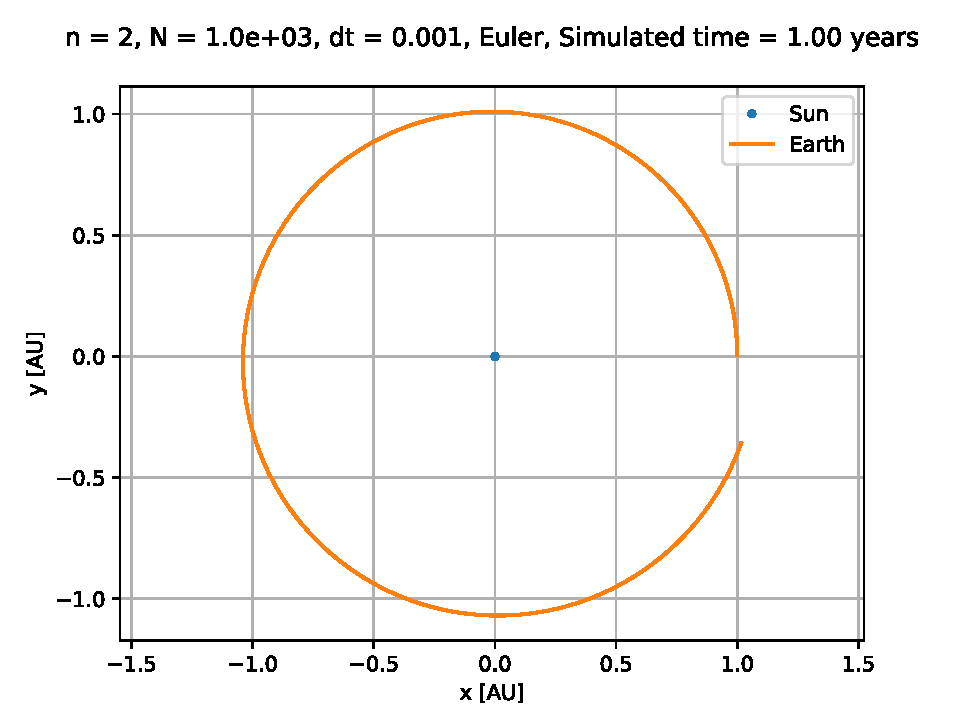
\includegraphics[width=\columnwidth]{../data/figures/sun-earth-3c/se_dt1e-3_fe_orbit2D.pdf}
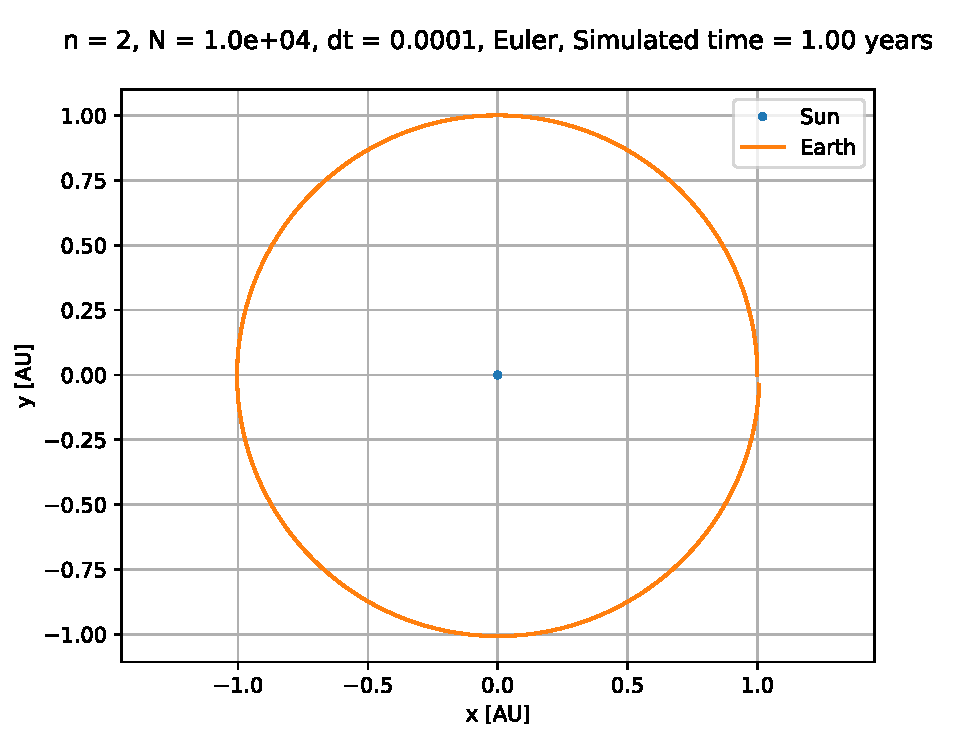
\includegraphics[width=\columnwidth]{../data/figures/sun-earth-3c/se_dt1e-4_fe_orbit2D.pdf}
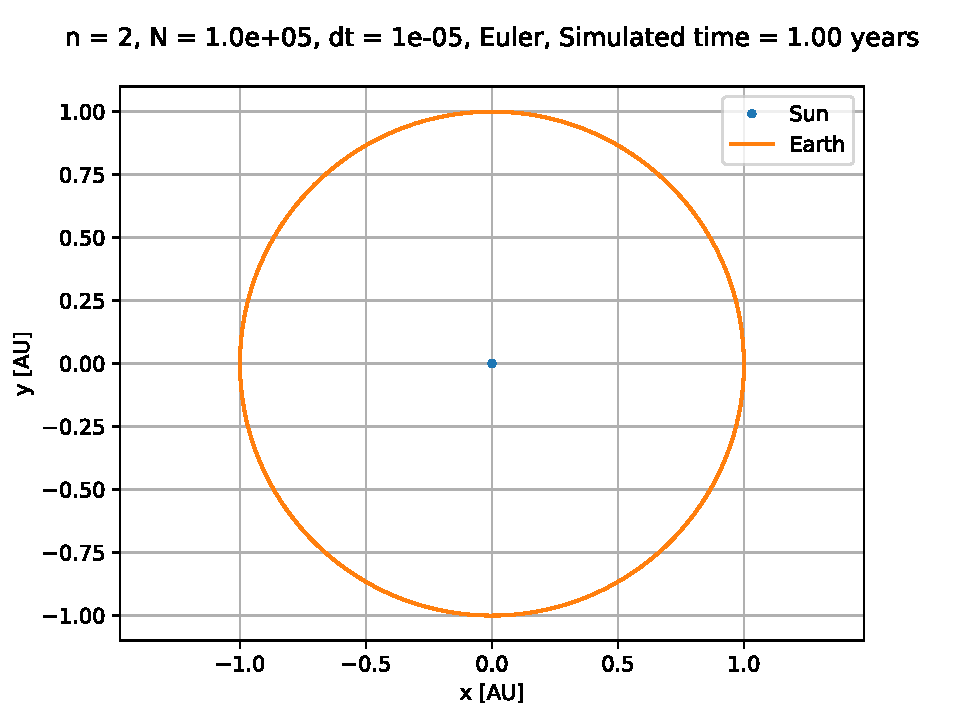
\includegraphics[width=\columnwidth]{../data/figures/sun-earth-3c/se_dt1e-5_fe_orbit2D.pdf}
\caption{This figure contains plots of simulated orbits of the Earth around the Sun for three different timesteps (denoted dt in the plots). These three simulations used the forward Euler method of integration (see section \hyperref[sec:II]{II} for details on the method and section \hyperref[sec:III]{III} for details on the simulation). In the title of the plot some variables are listed: n is the number of bodies, N the number of timesteps, dt the timestep, and the rest is self-explanatory.}
\label{fig:se-fe-orbits}
\end{figure}

\begin{figure}[H]
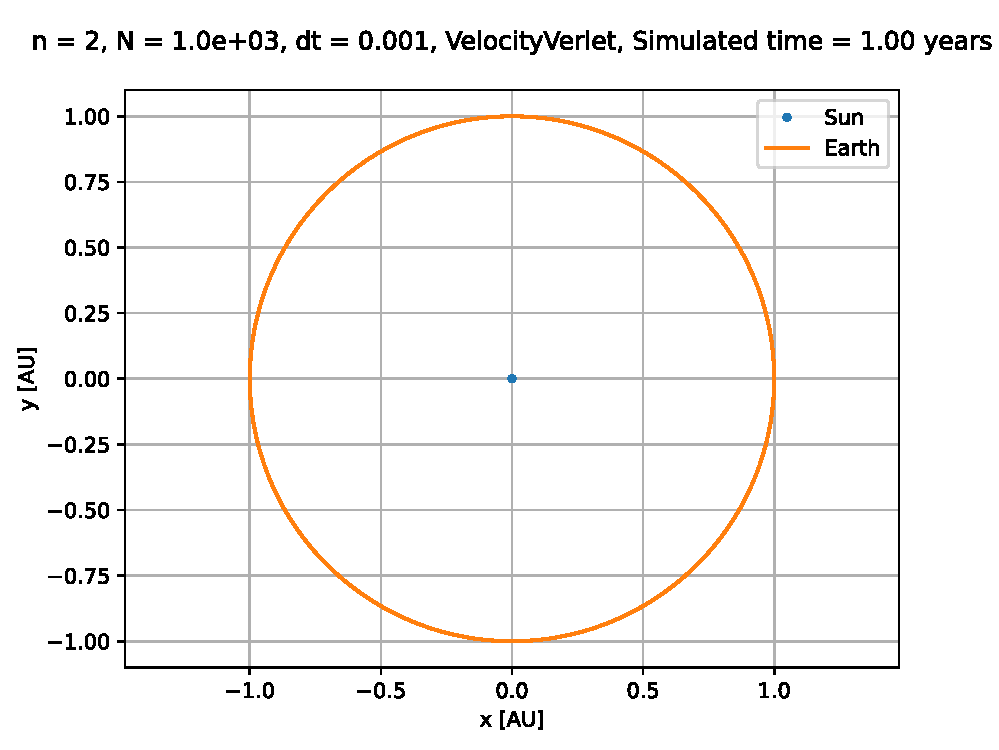
\includegraphics[width=\columnwidth]{../data/figures/sun-earth-3c/se_dt1e-3_vv_orbit2D.pdf}
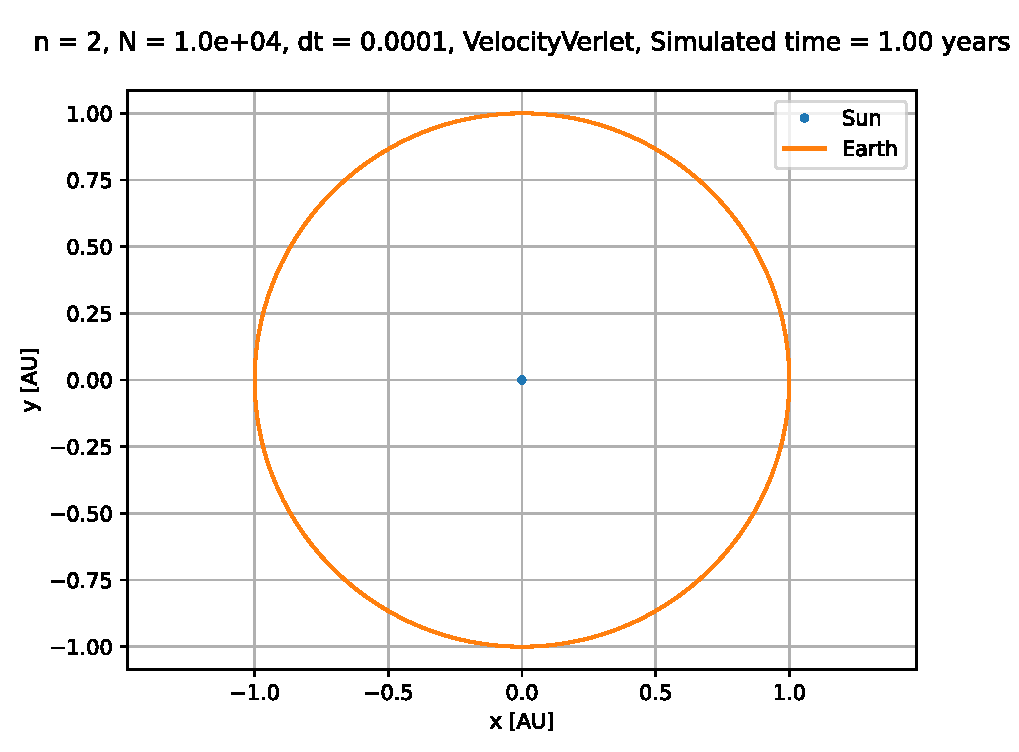
\includegraphics[width=\columnwidth]{../data/figures/sun-earth-3c/se_dt1e-4_vv_orbit2D.pdf}
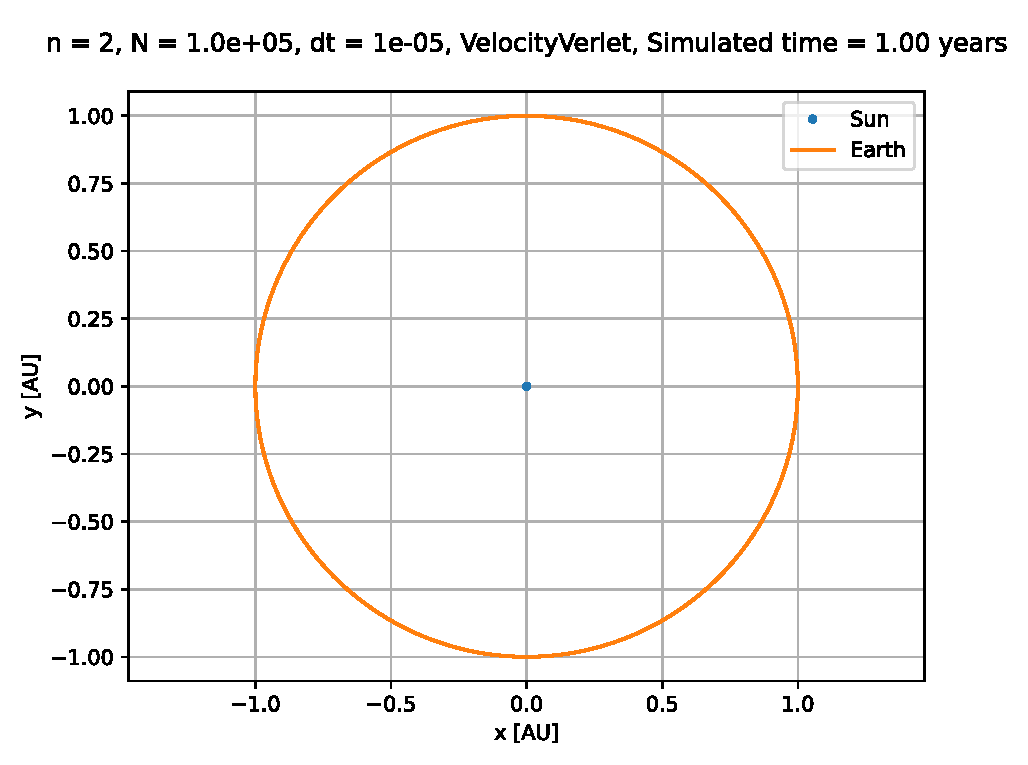
\includegraphics[width=\columnwidth]{../data/figures/sun-earth-3c/se_dt1e-5_vv_orbit2D.pdf}
\caption{This figure contains plots of simulated orbits of the Earth around the Sun for three different timesteps (denoted dt in the plots). These three simulations used the velocity Verlet method of integration (see section \hyperref[sec:II]{II} for details on the method and section \hyperref[sec:III]{III} for details on the simulation). In the title of the plot some variables are listed: n is the number of bodies, N the number of timesteps, dt the timestep, and the rest is self-explanatory.}
\label{fig:se-vv-orbits}
\end{figure}

\begin{table}
\caption{Table containing standard deviation of the total energy as a percentage of the mean total energy in the simulations described in section \hyperref[sec:IV:b]{IV.B}. The column labeled "Forward Euler" corresponds to the simulations performed with the forward Euler algorithm, and the column labeled "Velocity Verlet" corresponds to the simulationgs performed with the velocity Verlet algorithm.}
\begin{tabular}{|c|c|c|}
\hline
Timestep [years] & Forward Euler & Velocity Verlet \\
\hline
$10^{-3}$ & 1.97 \% & \num{4.28e-04} \% \\
$10^{-4}$ & 0.224 \% & \num{5.18e-04} \% \\
$10^{-5}$ & \num{2.28e-02} \% & \num{5.10e-04} \% \\
\hline
\end{tabular}
\label{table:se-3c-energydeviation}
\end{table}

\begin{figure}[H]
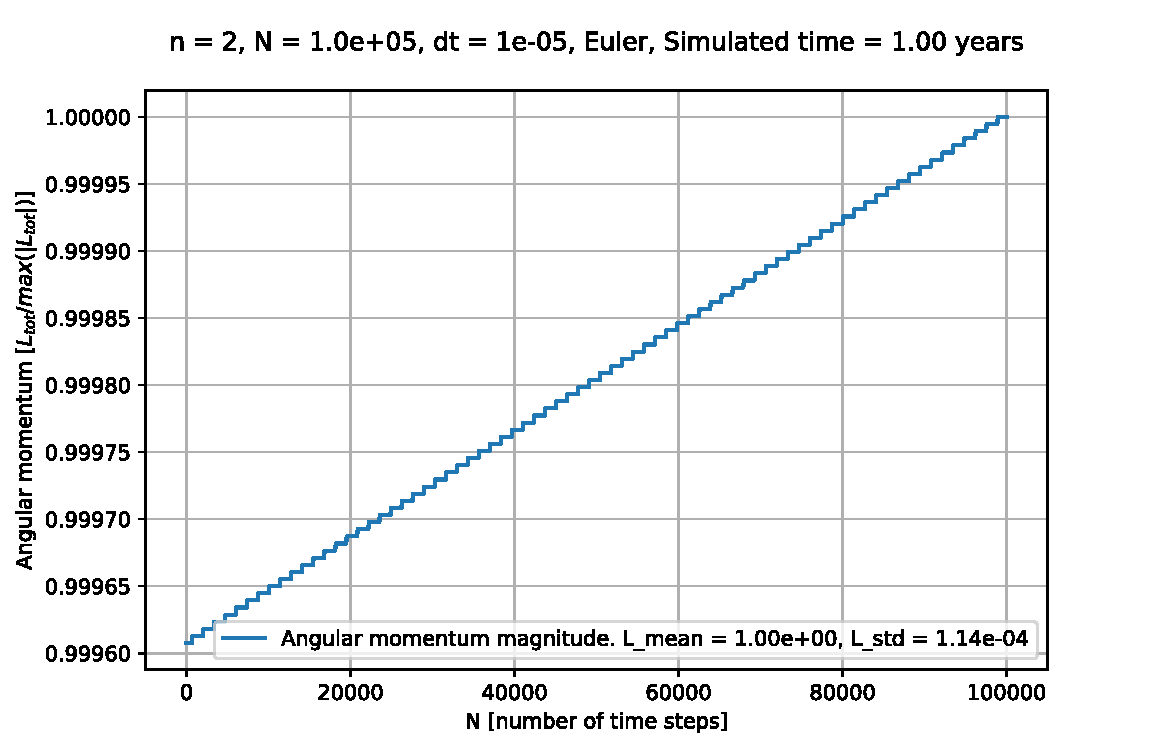
\includegraphics[width=\columnwidth]{../data/figures/sun-earth-3c/se_dt1e-5_fe_angmom.pdf}
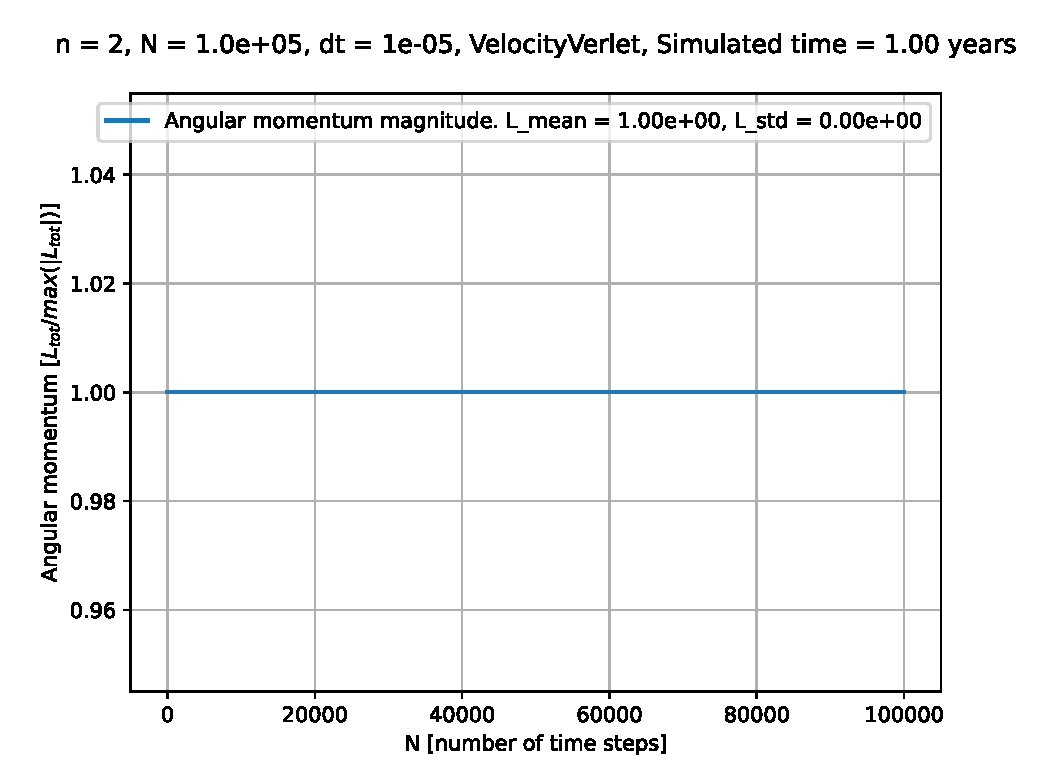
\includegraphics[width=\columnwidth]{../data/figures/sun-earth-3c/se_dt1e-5_vv_angmom.pdf}
\caption{This figure contains two plots showing the norm of the total angular momentum $L$, scaled so that it's maximum value is 1, as it develops during two simulations with Earth and the Sun. Both simulations were ran with a timestep $\Delta t = \num{1e-05}$, but one of them used the forward Euler algorithm, and the other the velocity Verlet algorithm (as indicated in the plot). The mean and standard deviation of $L$ is listed in the legend text.   }
\label{fig:se-3c-angmom}
\end{figure}


\subsection{Simulations of Earth and the Sun with another kind of force} \label{sec:IV:c}

We ran simulations of the system with Earth and the Sun with the force given \eqref{eq:beta_gengrav}, for different choices of the parameter $\beta$. These simulations were all performed with the velocity Verlet algorithm, the timestep set to $\Delta t = \num{1e-06}$ and the amount of timesteps $N = \num{1e+07}$. First we ran simulations with the same initial conditions as in section. In this case all the plots of the orbits remained roughly the same for any choice of $\beta$ between $2$ and $3$ and thus we only include a plot of the orbit with $\beta=2.667$ which can be seen along with a plot showing potential, kinetic, and total energy in figure \ref{fig:beta-se-orbit-energy}.


\begin{figure}[H]
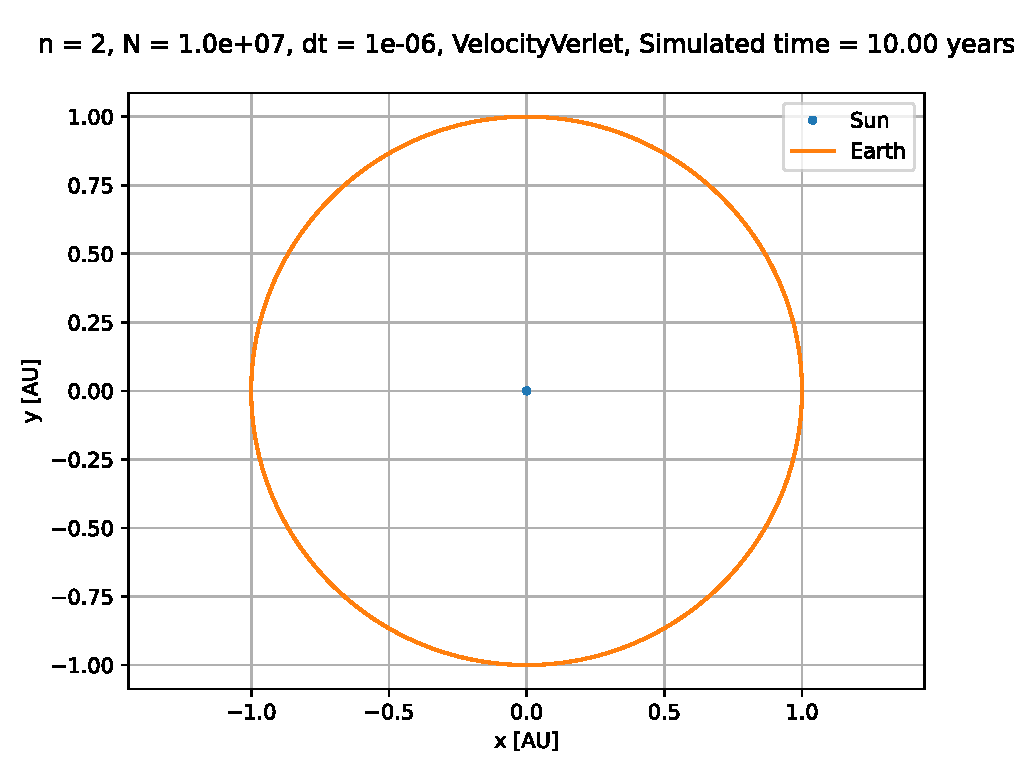
\includegraphics[width=\columnwidth]{../data/figures/varyingbeta/se_beta2667_vv_orbits2D.pdf}
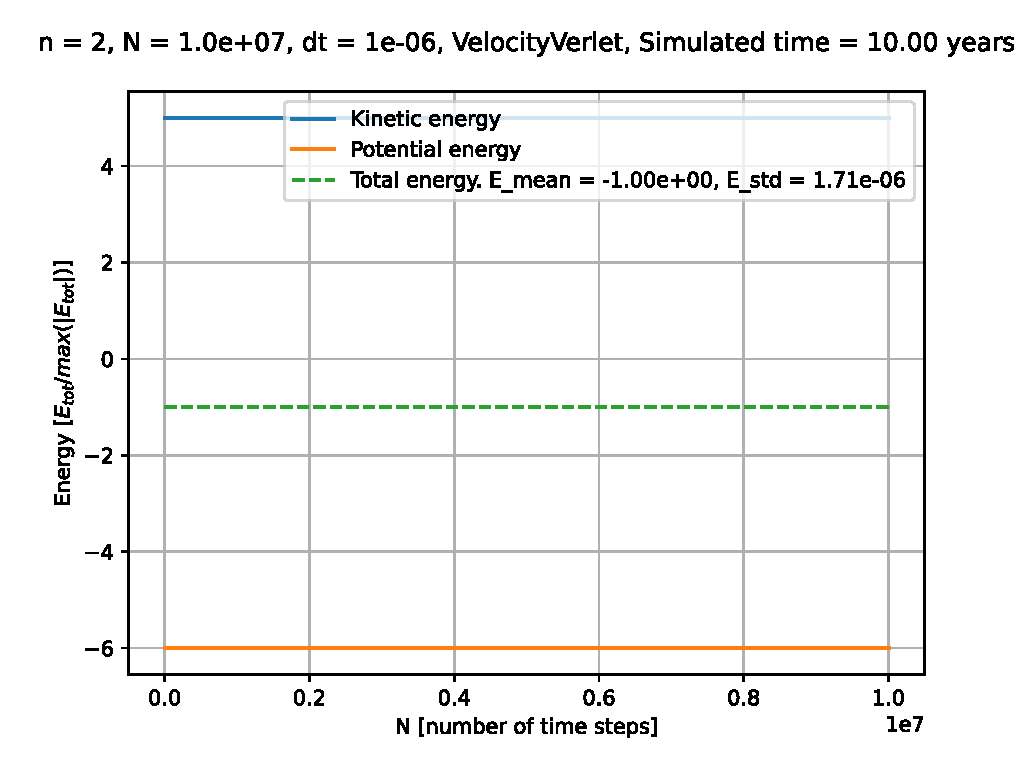
\includegraphics[width=\columnwidth]{../data/figures/varyingbeta/se_beta2667_vv_energy.pdf}
\caption{Figure containing two plots. The first plot shows the orbit of Earth around the Sun with the force interaction given by \eqref{eq:beta_gengrav}, where the parameter $\beta = 2.667$. The second plot shows potential, kinetic, and total energy in the same simulation.} 
\label{fig:beta-se-orbit-energy}
\end{figure}

We also ran simulations with the same initial conditions, except that we set the initial velocity of the earth to be 5 AU/year instead of $2\pi$ AU/year. With a regular gravitational interaction this corresponds to elliptical orbits. We ran these simulations with $\beta = 2$, $\beta = 2.333$, $\beta = 2.667$ and $\beta = 3$. Setting $\beta=2$ is the same as a regular gravitational interaction. We show plots of the orbit and the energy in this case in figure \ref{fig:beta2_peturbed}. The angular momentum remains a constant and is thus not shown. Plots of the orbit and energies in the case where $\beta = 2.333$ are shown in figure \ref{fig:beta233_peturbed}. The angular momentum remained a constant here as well and is thus not shown. Plots of the orbit and energies in the case where $\beta = 2.667$ are shown in figure \ref{fig:beta2667_peturbed}. The angular momentum remained constant here as well. Plots of the orbits, energies, and angular momentum in the case where $\beta = 3$ are shown in figure \ref{fig:beta3_peturbed}. The plot of the energies was zoomed in around the relevant portion of the plot. 

\begin{figure}[H]
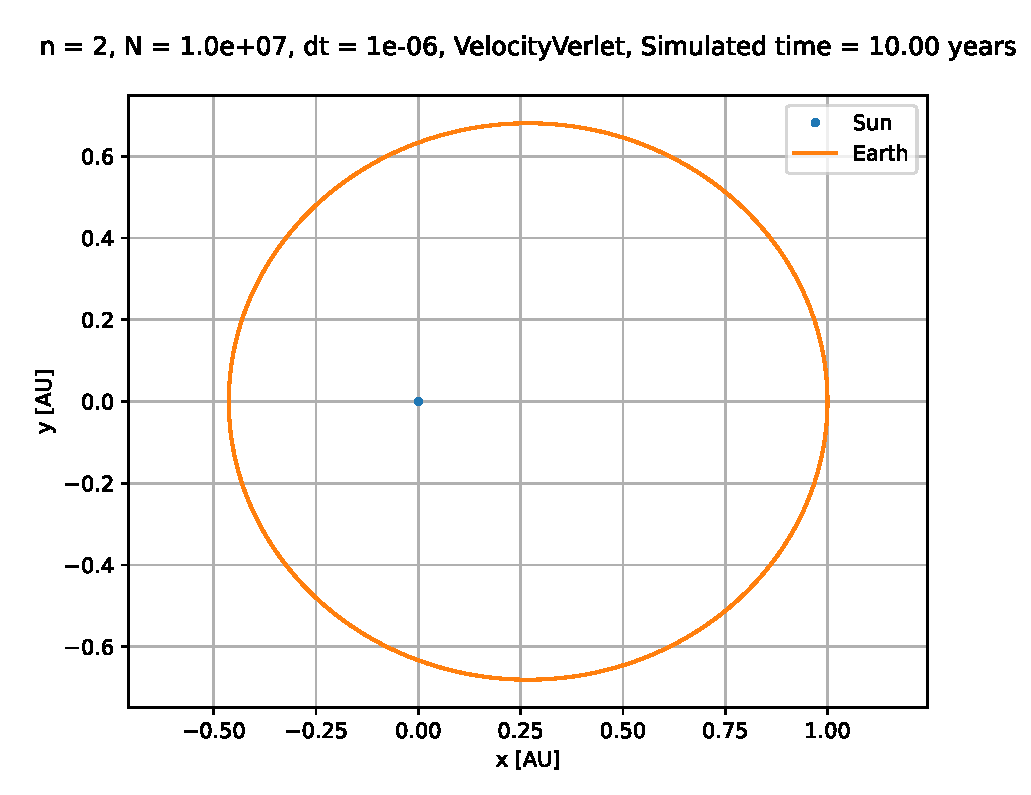
\includegraphics[width=\columnwidth]{../data/figures/varyingbeta/se_peturbed_beta2_vv_orbits2D.pdf}
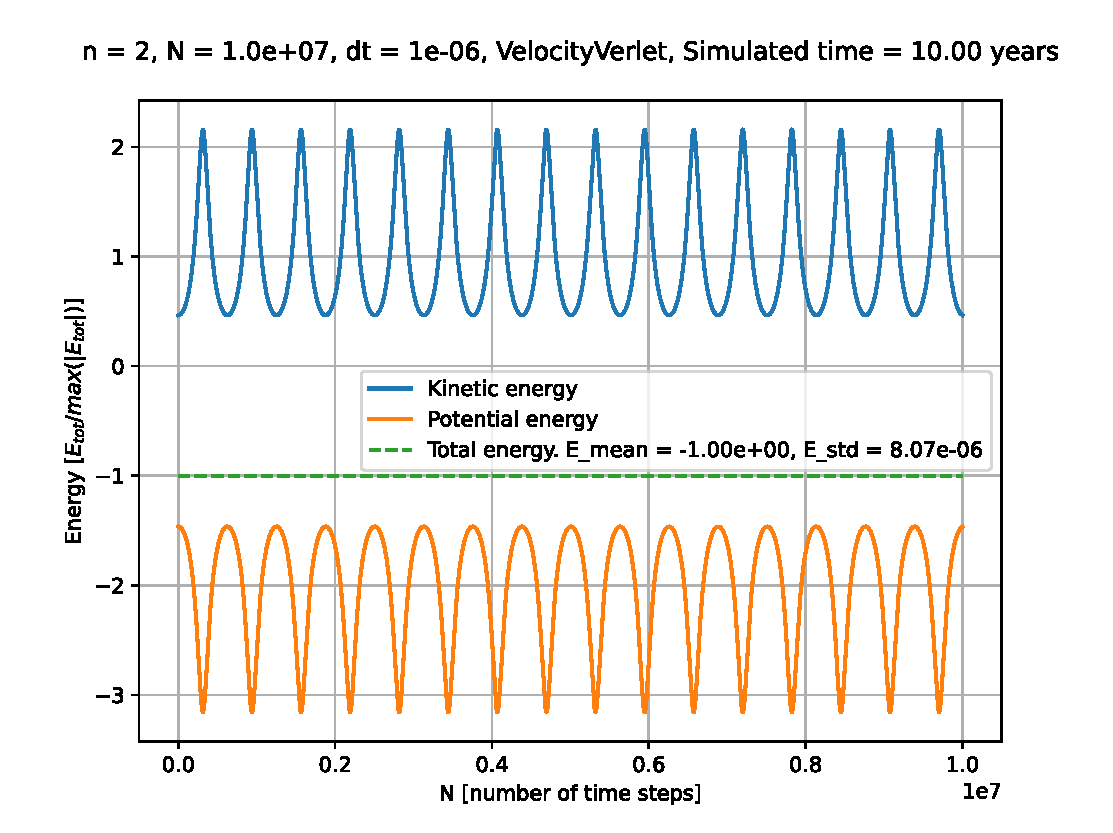
\includegraphics[width=\columnwidth]{../data/figures/varyingbeta/se_peturbed_beta2_vv_energy.pdf}
\caption{Figure contains a plot showing the simulated orbit of an Earth-like object orbiting around the Sun, and a plot showing potential, kinetic, and total energy for the system. The initial velocity has been altered (from the Earths initial velocity) so that the orbit is more elliptical. N is the amount of timesteps, dt is the timestep, and n is the number of bodies in the simulation.}
\label{fig:beta2_peturbed}
\end{figure}

\begin{figure}[H]
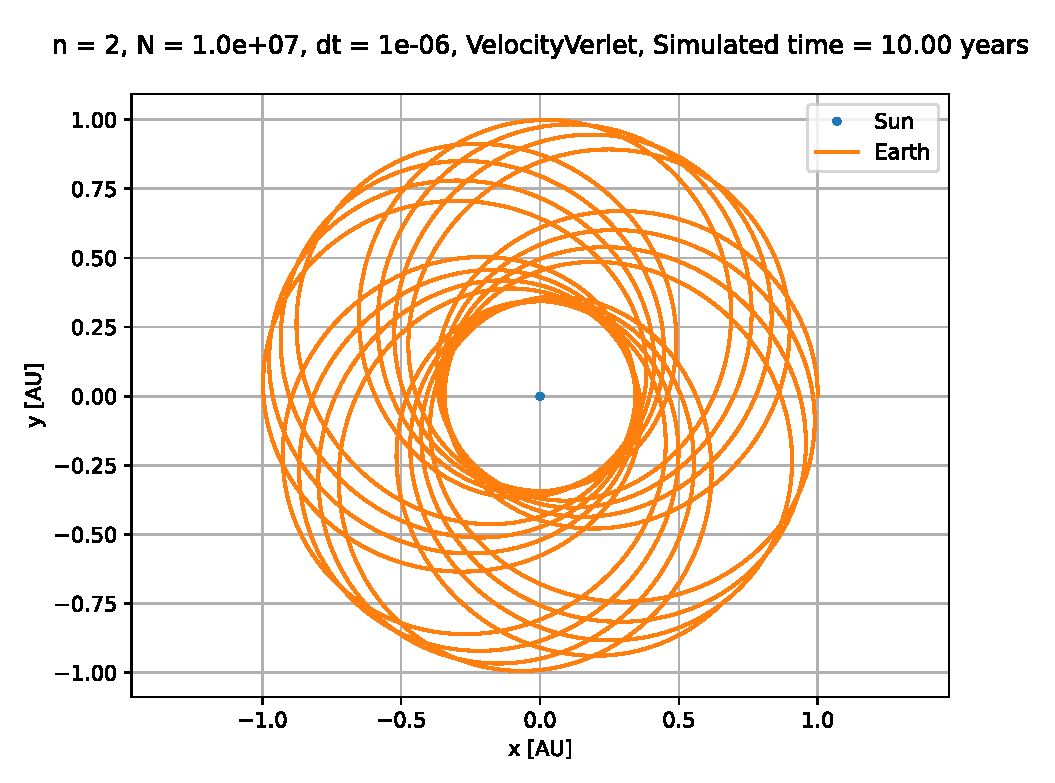
\includegraphics[width=\columnwidth]{../data/figures/varyingbeta/se_peturbed_beta233_vv_orbits2D.pdf}
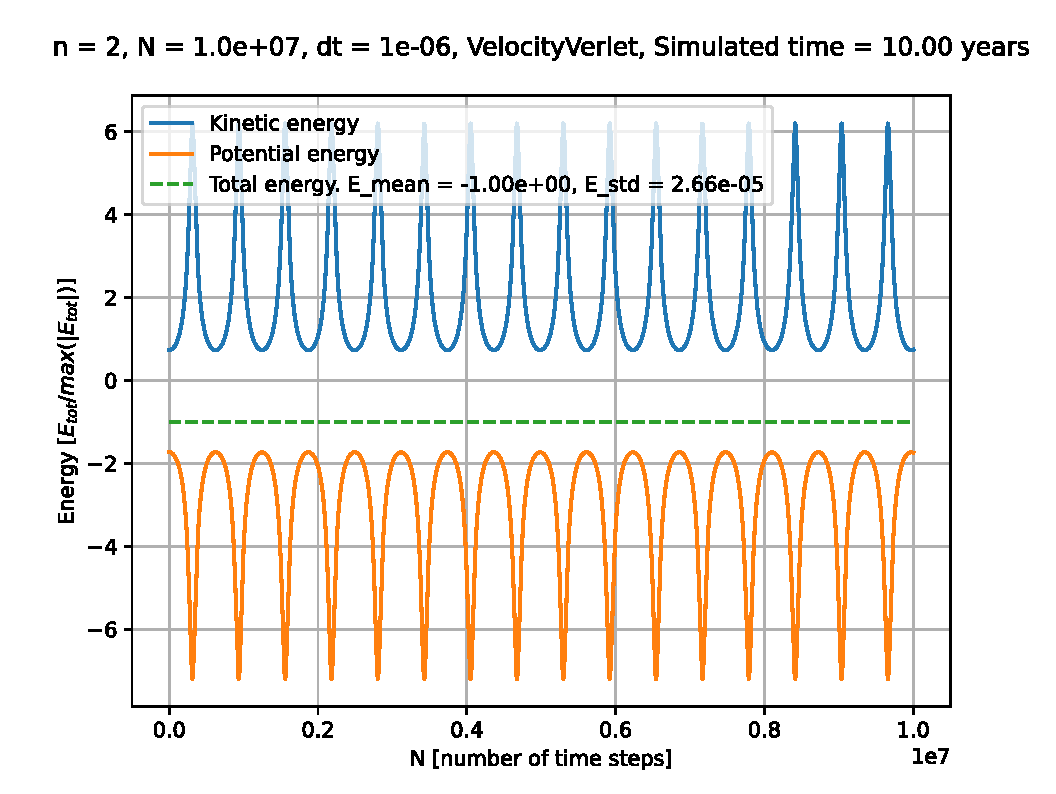
\includegraphics[width=\columnwidth]{../data/figures/varyingbeta/se_peturbed_beta233_vv_energy.pdf}
\caption{Figure contains a plot showing the simulated orbit of an Earth-like object orbiting around the Sun with a modified gravitational interaction (\eqref{eq:beta_gengrav} with $\beta = 2.333$), and a plot of the potential, kinetic, and total energy for this system. The initial velocity has been altered from the Earths initial velocity. N is the amount of timesteps, dt is the timestep, and n is the number of bodies in the simulation.}
\label{fig:beta233_peturbed}
\end{figure}

\begin{figure}[H]
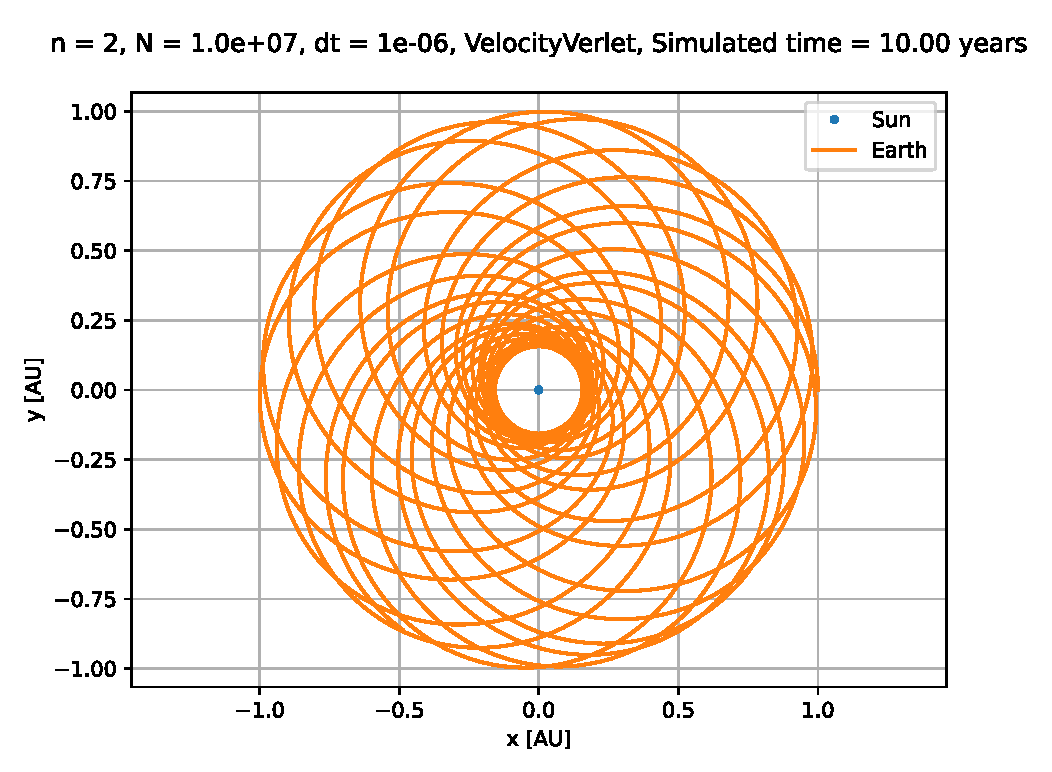
\includegraphics[width=\columnwidth]{../data/figures/varyingbeta/se_peturbed_beta2667_vv_orbits2D.pdf}
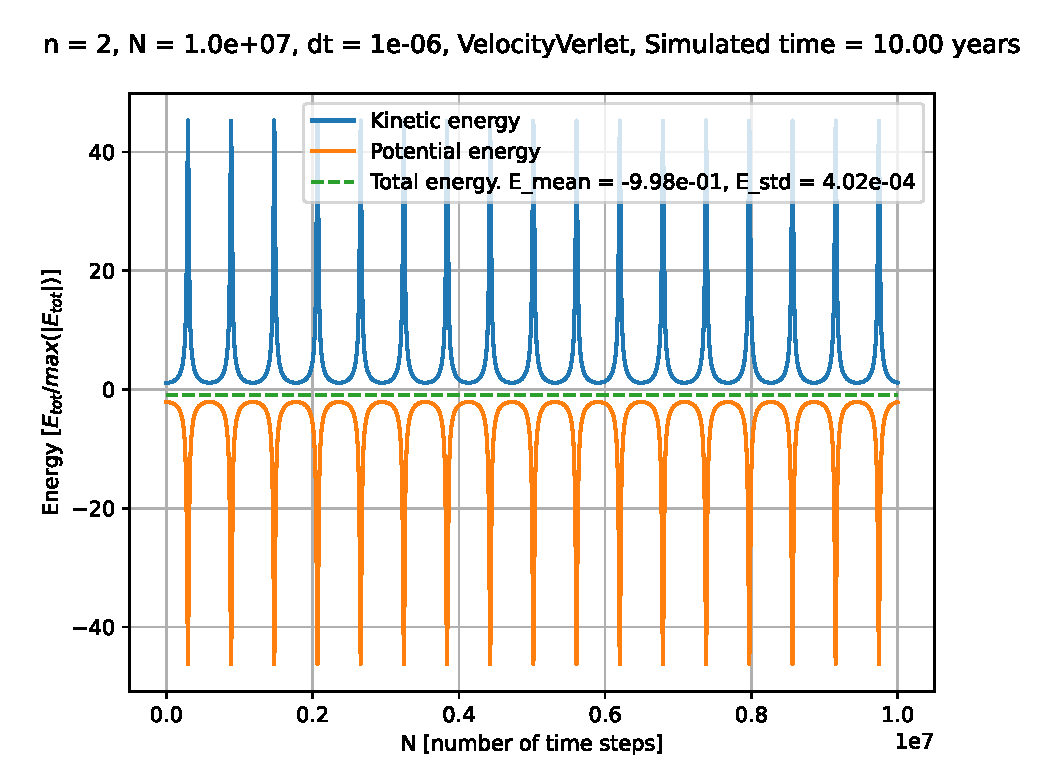
\includegraphics[width=\columnwidth]{../data/figures/varyingbeta/se_peturbed_beta2667_vv_energy.pdf}
\caption{Figure contains a plot showing the simulated orbit of an Earth-like object orbiting around the Sun with a modified gravitational interaction (\eqref{eq:beta_gengrav} with $\beta = 2.667$), and a plot of the potential, kinetic, and total energy for this system. The initial velocity has been altered from the Earths initial velocity. N is the amount of timesteps, dt is the timestep, and n is the number of bodies in the simulation.}
\label{fig:beta2667_peturbed}
\end{figure}

\begin{figure}[H]
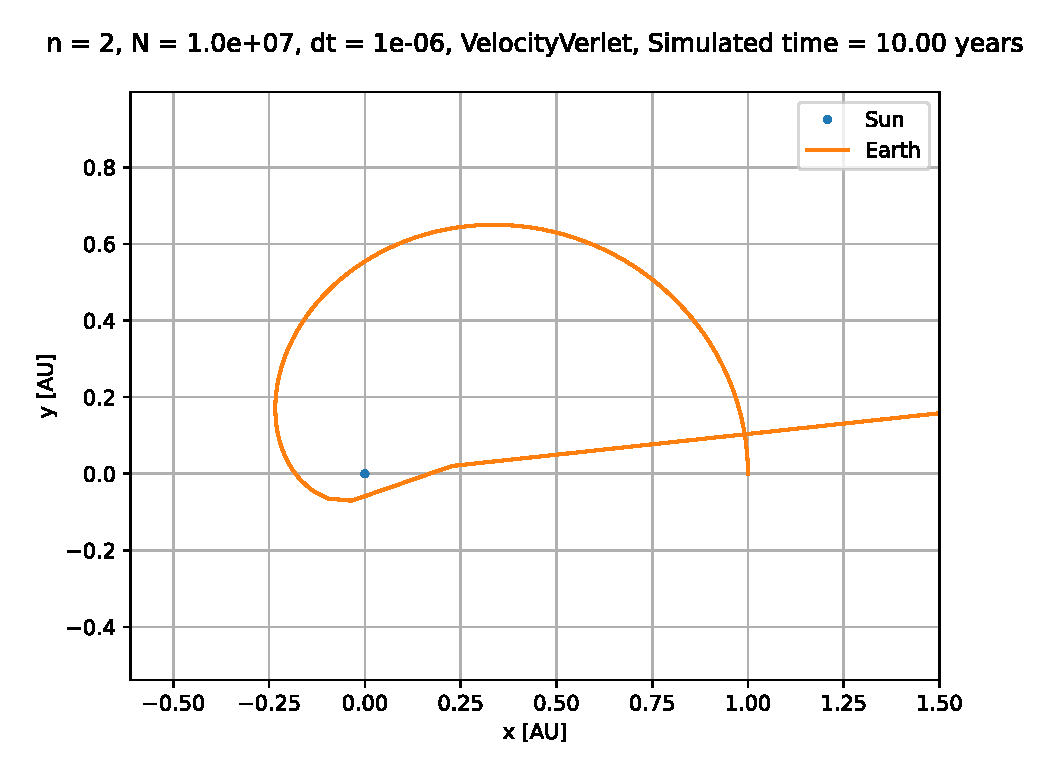
\includegraphics[width=\columnwidth]{../data/figures/varyingbeta/se_peturbed_beta3_vv_orbits2D.pdf}
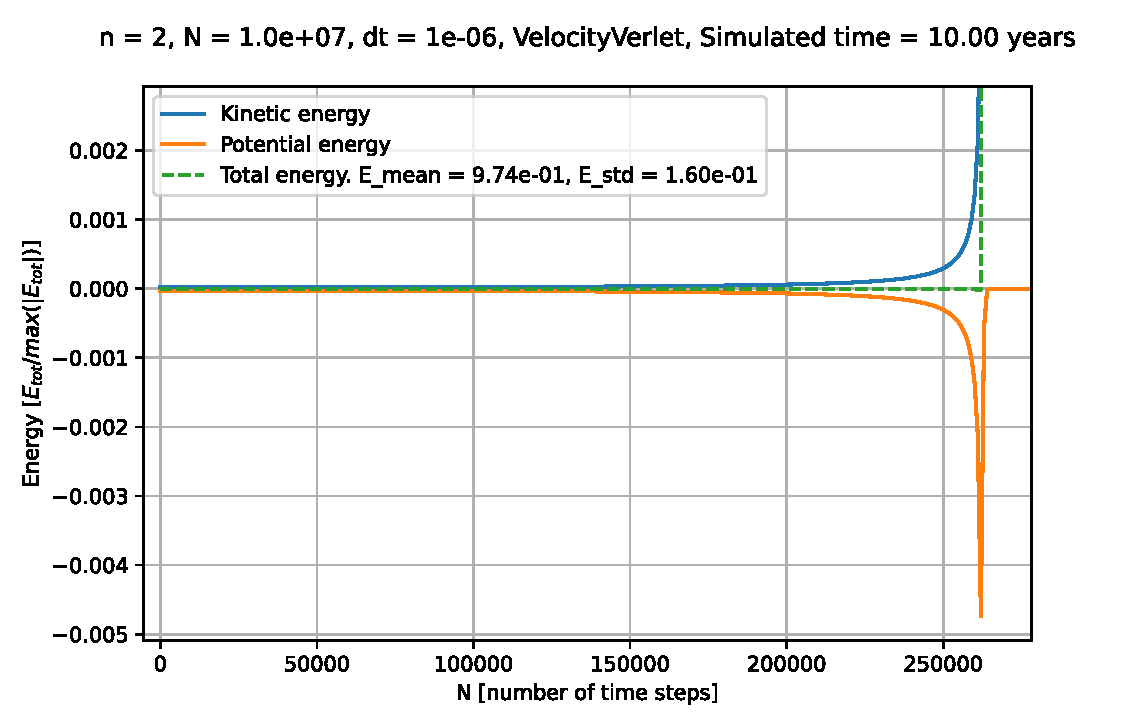
\includegraphics[width=\columnwidth]{../data/figures/varyingbeta/se_peturbed_beta3_vv_energy_zoomed.pdf}
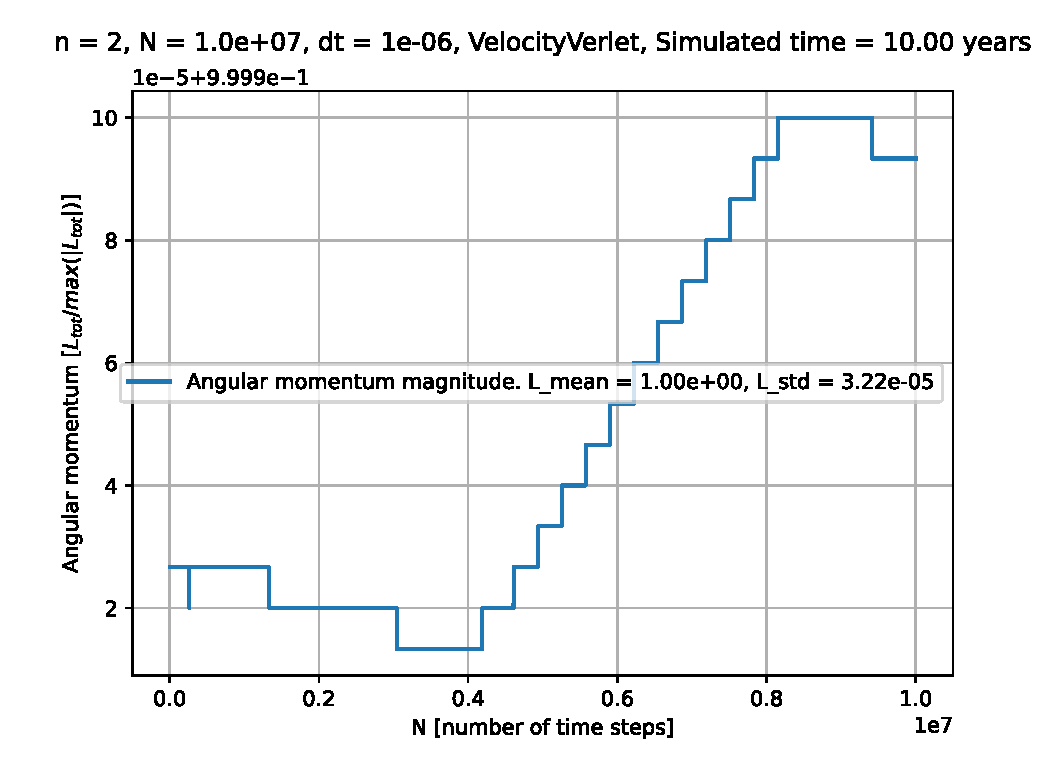
\includegraphics[width=\columnwidth]{../data/figures/varyingbeta/se_peturbed_beta3_vv_angmom.pdf}
\caption{Figure contains a plot showing the simulated orbit of an Earth-like object orbiting around the Sun with a modified gravitational interaction (\eqref{eq:beta_gengrav} with $\beta = 3$), a plot of the potential, kinetic, and total energy, and a plot of the norm of the total angular momentum of this system. Note that the plot of the energies is zoomed in around a relevant part, as the rest of the plot would be unreadable. The initial velocity has been altered from the Earths initial velocity. N is the amount of timesteps, dt is the timestep, and n is the number of bodies in the simulation.}
\label{fig:beta3_peturbed}
\end{figure}


\subsection{Simulations with velocity close to escape velocity} \label{sec:IV:d}

We ran simulations with Earth and the Sun, where we set Earths velocity to values close to the escape velocity in the Sun's gravitational field. The escape velocity of Earth in this case was found in section \hyperref[sec:II:e]{II.E} and the escape velocity itself is listed in \eqref{eq:esc_sun_1au}. All the simulations were ran with $N = \num{1e+07}$ timesteps and timestep $\Delta t = \num{2.48e-05}$. We needed to simulate for a sufficient amoount of time so that we could verify that the Earth would or would not escape the gravitational field of the Sun, and we chose then a set of parameters such that the simulation time is approximately equal to the time it takes Pluto to complete a full orbit around the Sun, as that makes sense in terms of objects in our Solar System. We chose this as a baseline set of parameters in our simulations. We used the velocity Verlet algorithm as the method of numerical integration in these simulations.

The Sun is set to the origin of the system, and Earth starts $1$ AU away from the Sun along the $x$-axis, and a varying velocity in the $y$-direction. We showcase three simulations here where the velocity was chosen such that it was just below, exactly at, or just above the escape velocity. We ran a simulation with the initial velocity set to $v = 8.8$ AU/year, one with $v = 2\pi \sqrt{2} \approx 8.886$, and the last with $v = 9$ AU/year. Plots showing the orbit and energies in these simulations can be found in figures \ref{fig:escvel_88}, \ref{fig:escvel_exact} and \ref{fig:escvel_9} respectively.


\begin{figure}[H]
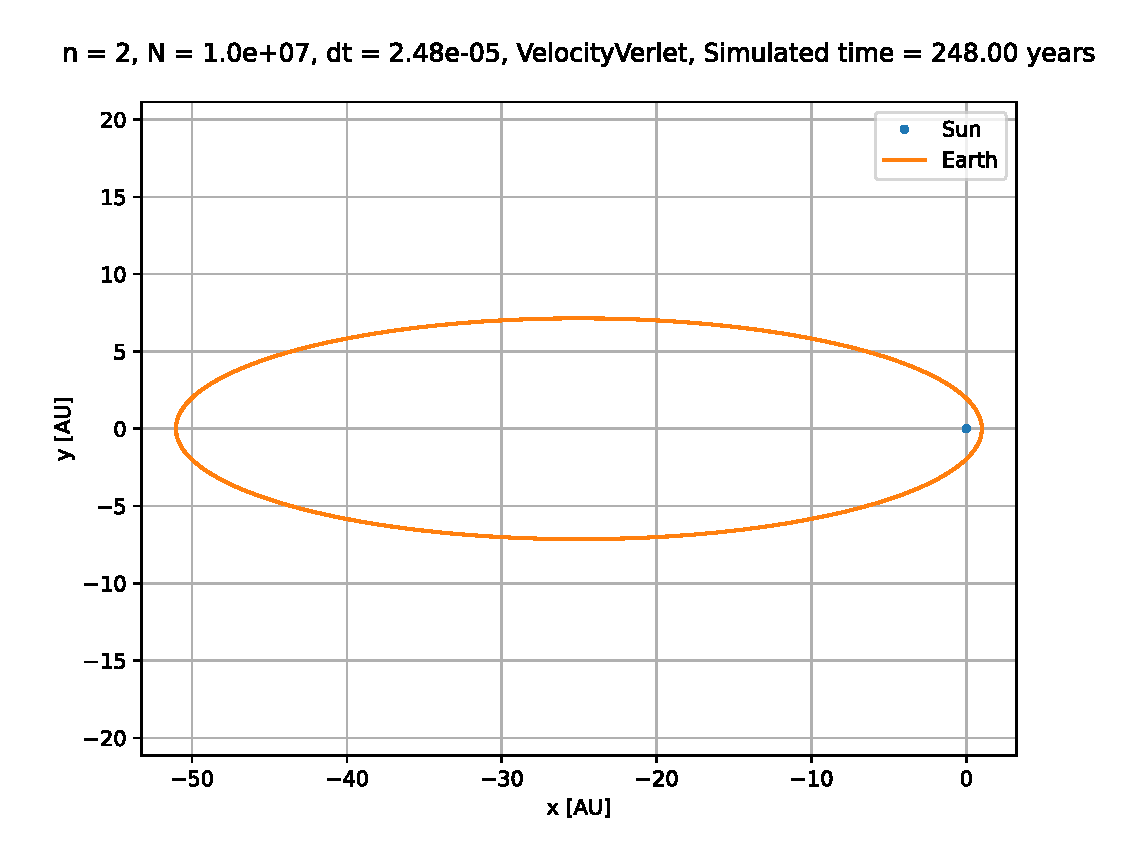
\includegraphics[width=\columnwidth]{../data/figures/escapevelocity/se_esc_8-8_orbit2D.pdf}
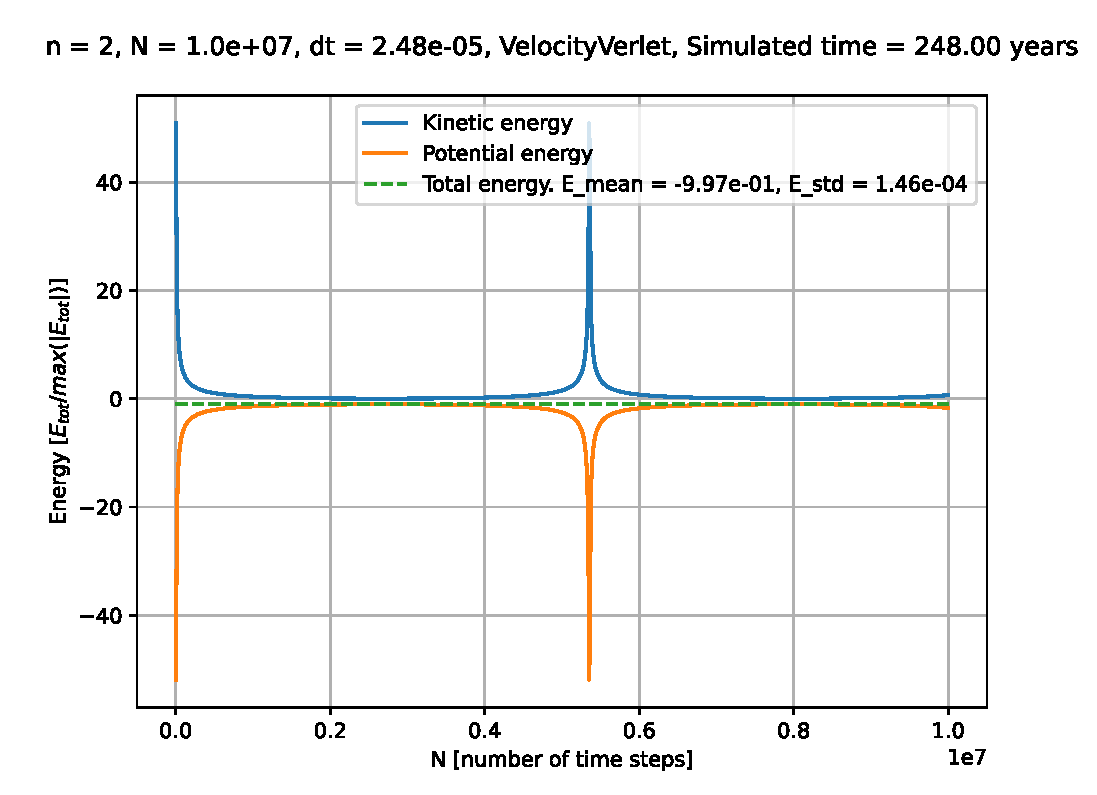
\includegraphics[width=\columnwidth]{../data/figures/escapevelocity/se_esc_8-8_energy.pdf}
\caption{This figure contains plots of the path the Earth took in a simulation with Earth and the Sun and the energy in this system. The initial conditions used are listed in section \hyperref[sec:IV:d]{IV.D}. N is the number of timesteps, dt the timestep, and n the number of bodies in the system.}
\label{fig:escvel_88}
\end{figure}

\begin{figure}[H]
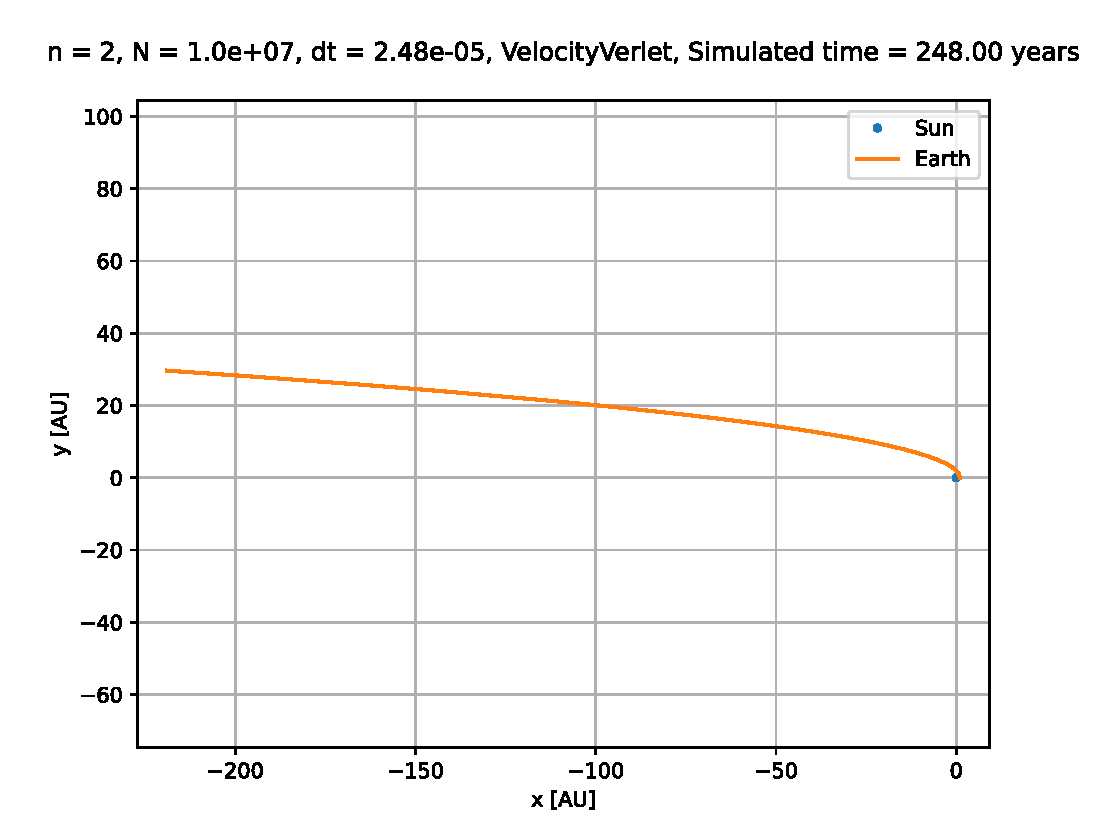
\includegraphics[width=\columnwidth]{../data/figures/escapevelocity/se_esc_exact_orbit2D.pdf}
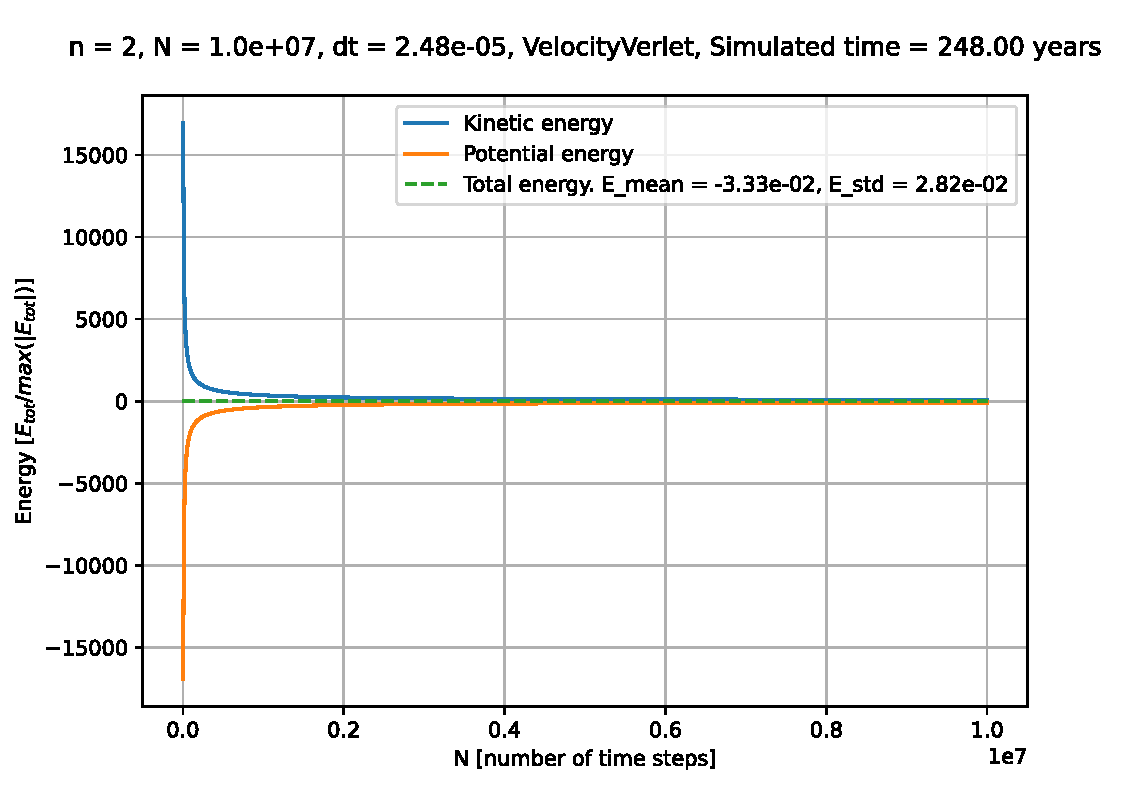
\includegraphics[width=\columnwidth]{../data/figures/escapevelocity/se_esc_exact_energy.pdf}
\caption{This figure contains plots of the path the Earth took in a simulation with Earth and the Sun and the energy in this system. The initial conditions used are listed in section \hyperref[sec:IV:d]{IV.D}. N is the number of timesteps, dt the timestep, and n the number of bodies in the system.}
\label{fig:escvel_exact}
\end{figure}

\begin{figure}[H]
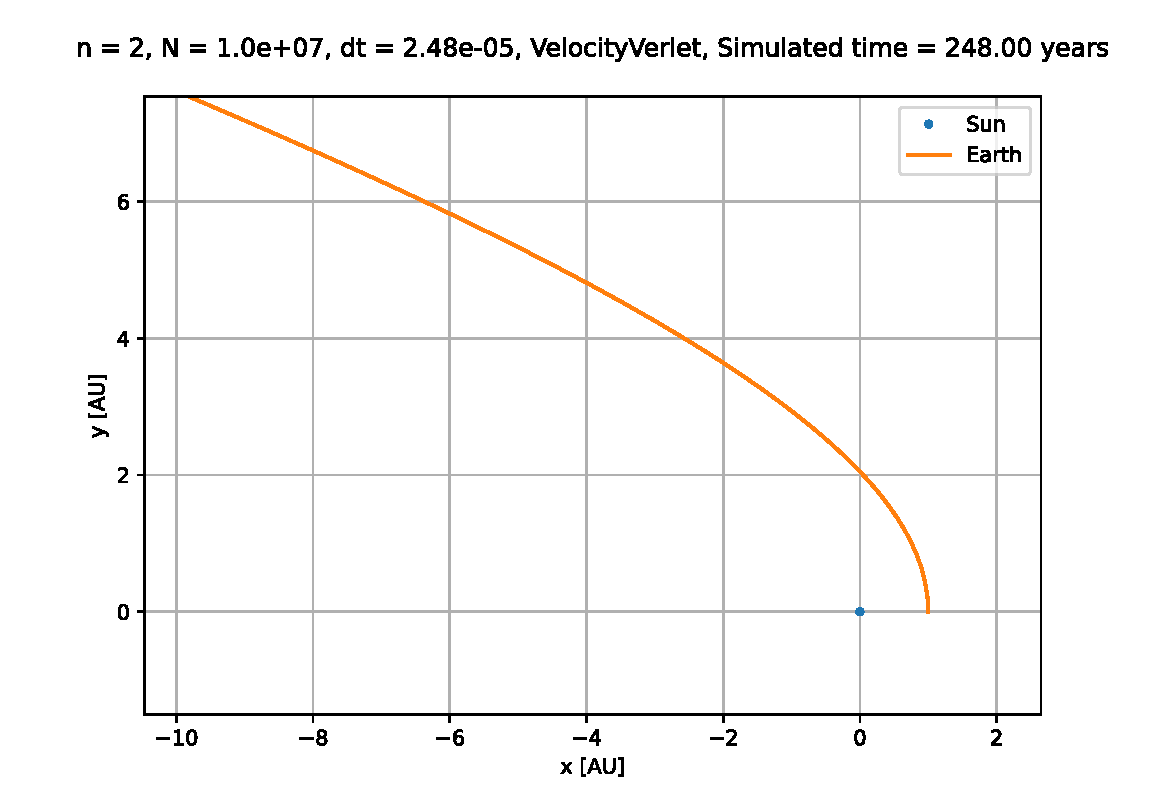
\includegraphics[width=\columnwidth]{../data/figures/escapevelocity/se_esc_9_orbit2D_zoomed.pdf}
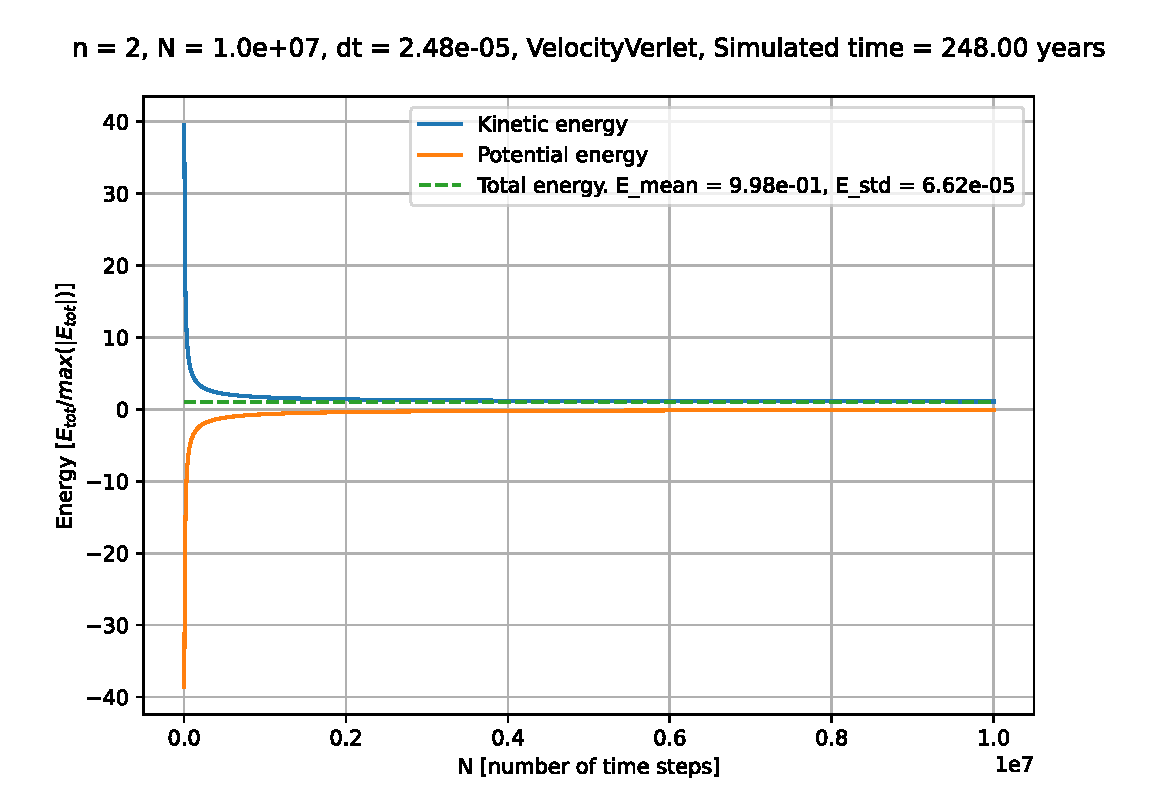
\includegraphics[width=\columnwidth]{../data/figures/escapevelocity/se_esc_9_energy.pdf}
\caption{This figure contains plots of the path the Earth took in a simulation with Earth and the Sun and the energy in this system. The initial conditions used are listed in section \hyperref[sec:IV:d]{IV.D}. N is the number of timesteps, dt the timestep, and n the number of bodies in the system.}
\label{fig:escvel_9}
\end{figure}



\subsection{Simulations of Earth, Jupiter and the Sun} \label{sec:IV:e}

We ran simulations with Earth, Jupiter and the Sun. The initial conditions were obtained using \citep{NASASolarInit}. Three simulations were performed with this system, one with the standard initial conditions, one with the mass of Jupiter being a factor 10 larger, and the last one with it being a factor $10^3$ larger. All the simulations were ran with $N=10^7$ timesteps, with steplength $\Delta t = \num{1.2e-06}$. This set of parameters was chosen so that Jupiter would complete a full orbit around the Sun. Plots of the resulting orbits can be found in figures \ref{fig:sej-standard}, \ref{fig:sej-10} and \ref{fig:sej-1000}. Which plots are shown is determined by readability. All of the plots in these figures are in the reference system of the Sun. The simulations were ran in the center of mass frame, and then transformed to the reference frame of the Sun when processing the data. In most cases the 3D plots are the best, as the simulations were all ran in three dimensions, but in some other cases the plots in the $xy$-plane are much easier to read, and give a better overview of the results. The angular momentum and total energy remained constant in all of these simulations, and thus plots of these were not included. 

\begin{figure}[H]
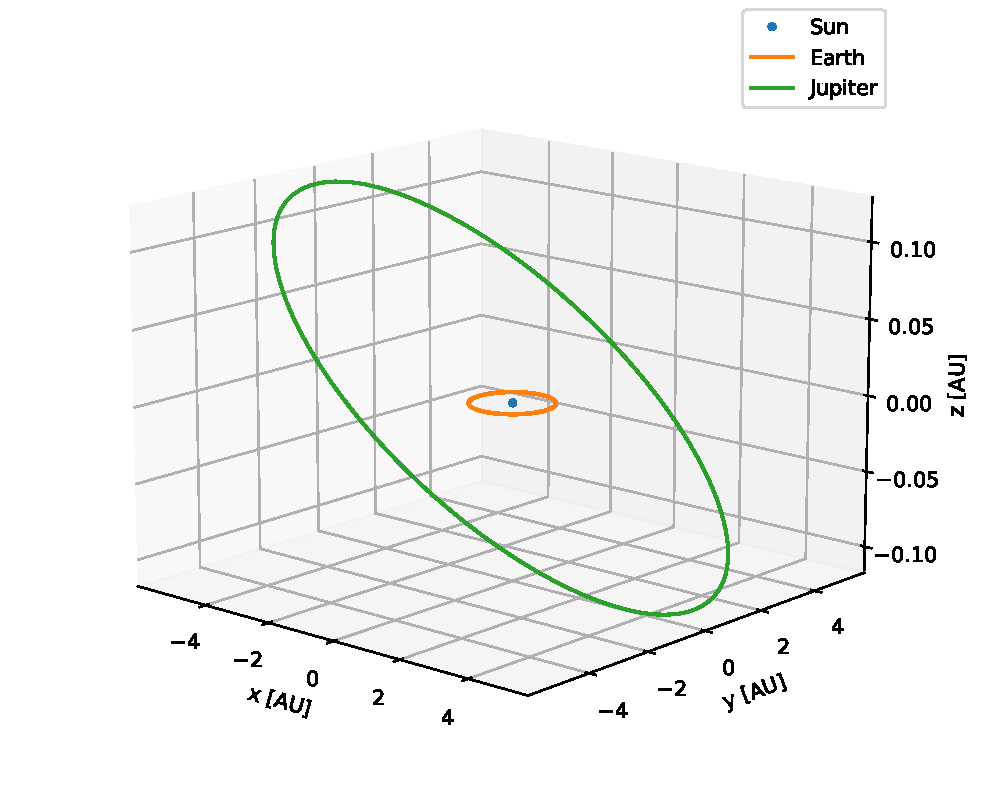
\includegraphics[width=\columnwidth]{../data/figures/sun-earth-jupiter/sej_1xM_vv_orbit3D.pdf}
\caption{This figure contains a 3D plot of the simulated orbits of Earth and Jupiter around the Sun. The simulation was ran with $N=10^7$ timesteps and steplength $\Delta t = \num{1.2e-06}$ years. Note that the axes in the plot are not equal, so the orbit of Jupiter is not as tilted as it may seem to be at first glance.}
\label{fig:sej-standard}
\end{figure}

\begin{figure}[H]
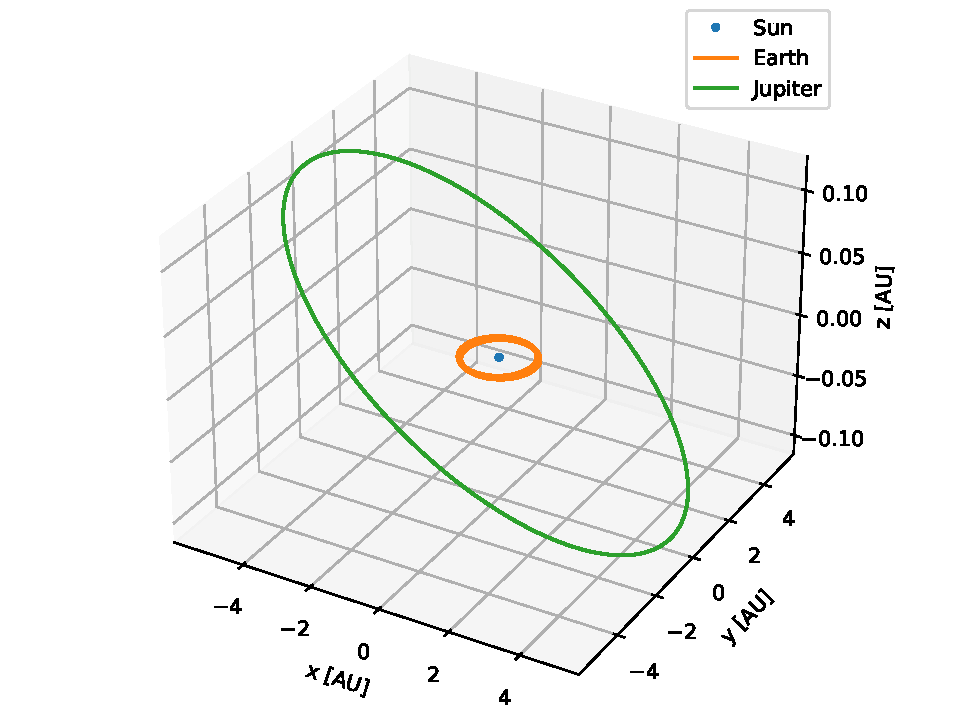
\includegraphics[width=\columnwidth]{../data/figures/sun-earth-jupiter/sej_10xM_vv_orbit3D.pdf}
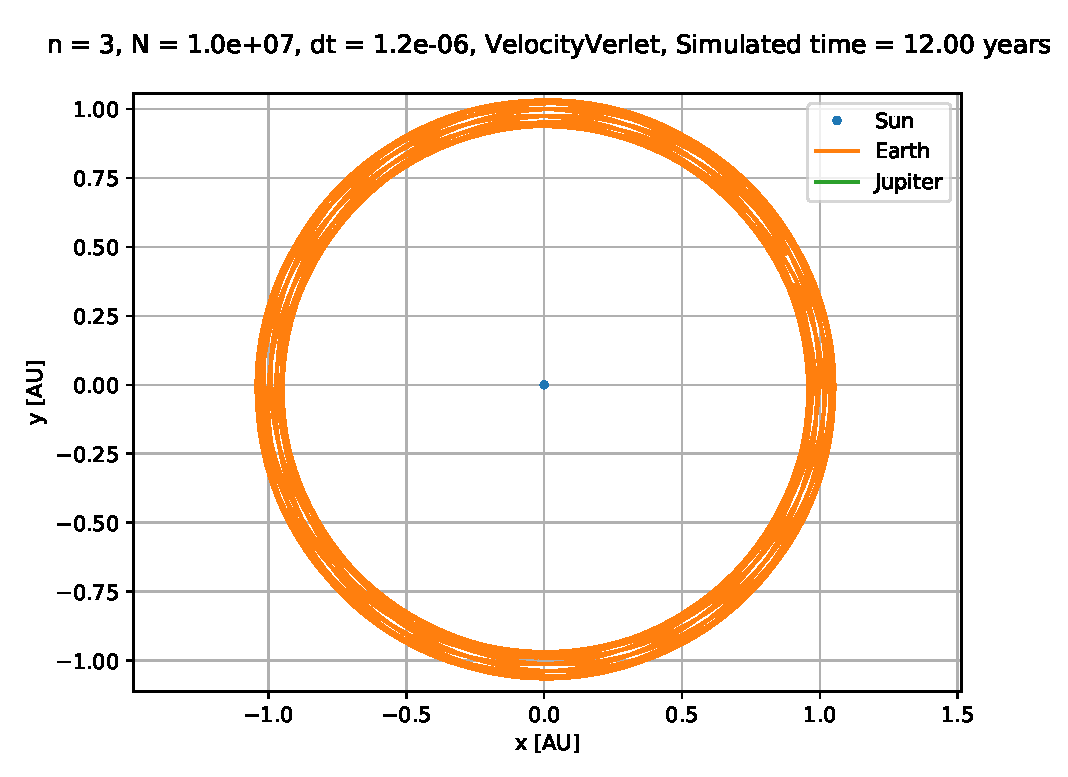
\includegraphics[width=\columnwidth]{../data/figures/sun-earth-jupiter/sej_10xM_vv_orbit2D_zoomed.pdf}
\caption{This figure contains a 3D plot of the simulated orbits of Earth and Jupiter (with Jupiters mass being set to be 10 times larger than it actually is) around the Sun, and another plot of the same simulation but zoomed in to better show Earths orbit in the $xy$-plane. The simulation was ran with $N=10^7$ timesteps and steplength $\Delta t = \num{1.2e-06}$ years. Note that the axes in the plot are not equal, so the orbit of Jupiter is not as tilted as it may seem to be at first glance.}
\label{fig:sej-10}
\end{figure}

\begin{figure}[H]
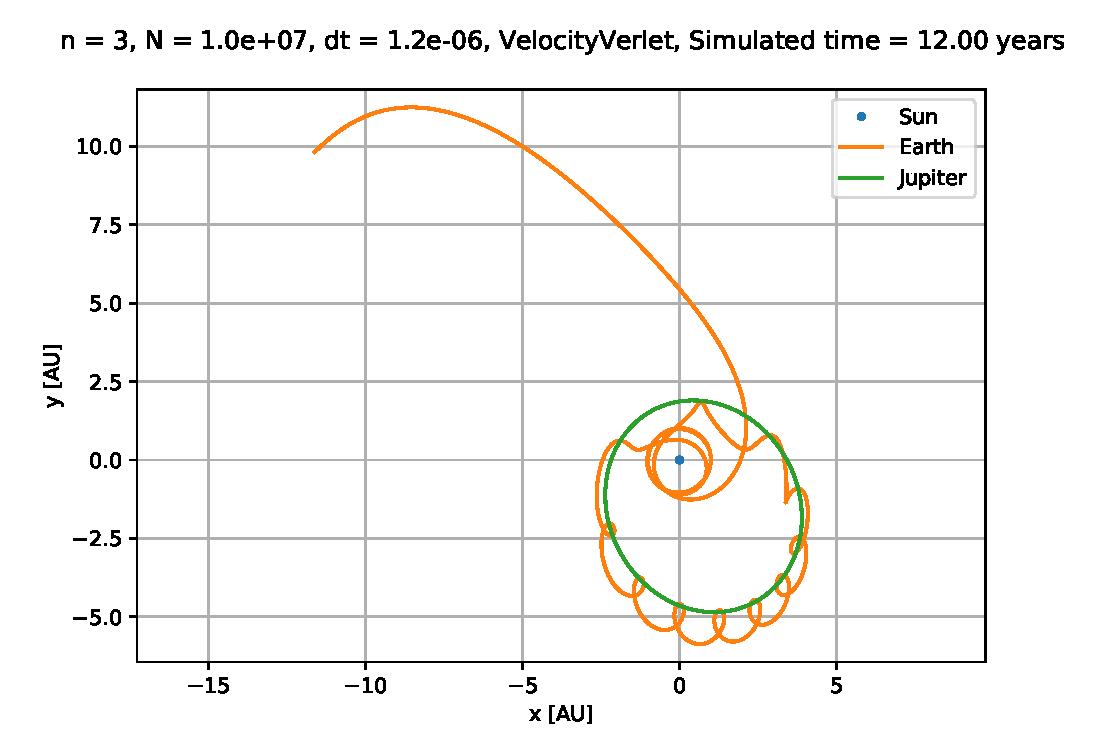
\includegraphics[width=\columnwidth]{../data/figures/sun-earth-jupiter/sej_1000xM_vv_orbit2D.pdf}
\caption{This figure contains a plot of the simulated orbits of Earth and Jupiter (with Jupiters mass being set to be $10^3$ times larger than it actually is) around the Sun in the $xy$-plane. The simulation was ran with $N=10^7$ timesteps and steplength $\Delta t = \num{1.2e-06}$ years.}
\label{fig:sej-1000}
\end{figure}



\subsection{Simulation of the Solar System} \label{sec:IV:f}

We ran a simulation of the planets of the Solar System, the Sun and Pluto. Hereby we refer to this system as just "the Solar System", even though we have not included all objects that are in the actual Solar System. The simulation had $N = 10^7$ timesteps and steplength $\Delta t = \num{2.48e-05}$. This set of parameters was chosen so that Pluto would complete a full revolution around the Sun. Plots of the resulting orbits is shown in figure \ref{fig:ss}. The initial conditions for this system was generated using \citep{NASASolarInit}.

\begin{figure}[H]
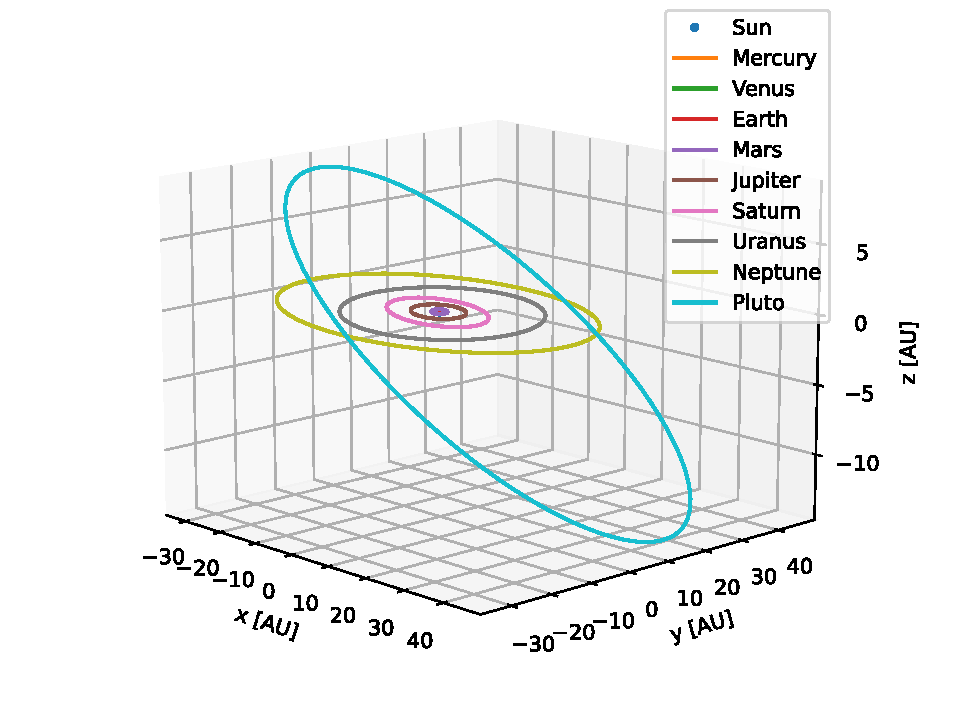
\includegraphics[width=\columnwidth]{../data/figures/sun_and_friends/ss_248_vv_orbits3D.pdf}
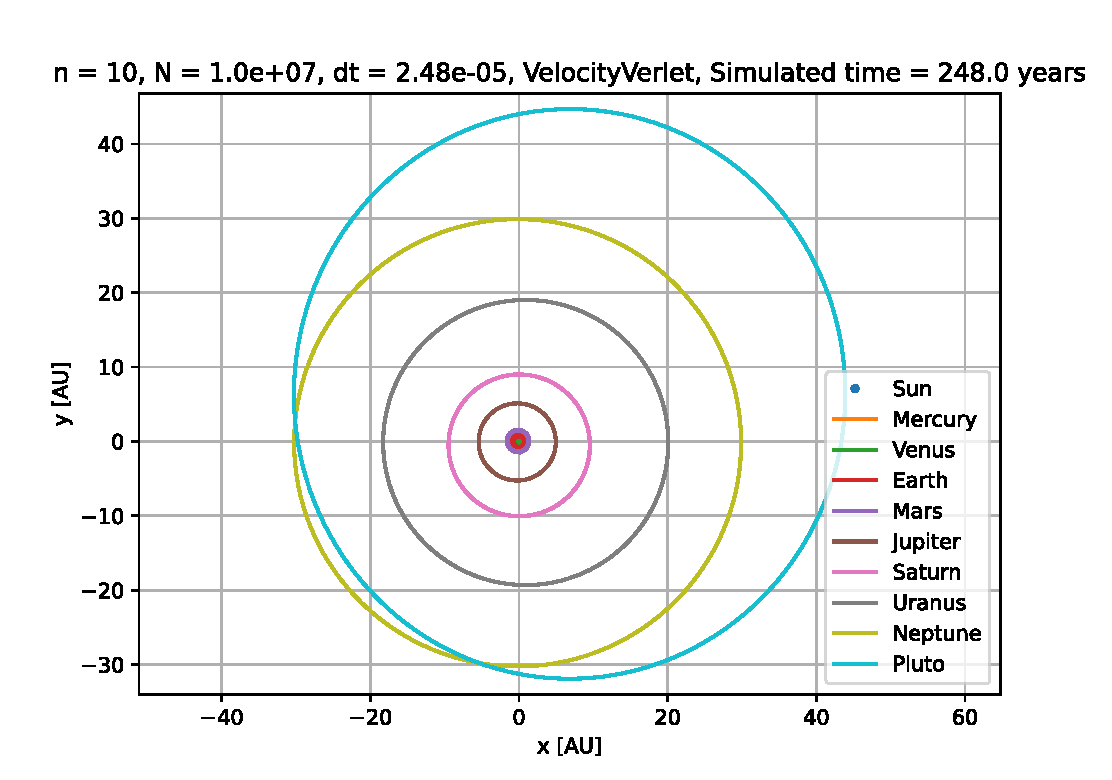
\includegraphics[width=\columnwidth]{../data/figures/sun_and_friends/ss_248_vv_orbits2D.pdf}
\caption{This figure contains a 3D plot of the simulated orbits of the planets (and Pluto) in the Solar System around the Sun. The simulation had $N = 10^7$ timesteps and steplength $\Delta t = \num{2.48e-05}$. Note that the axes are not equal. The figure also contains a plot of the orbits in the $xy$-plane.}
\label{fig:ss}
\end{figure}



\subsection{Calculating the perihelion precession of Mercury} \label{sec:IV:g}

We ran a simulation with Mercury and the Sun with the modified gravitational interaction given in \eqref{eq:grav_rel}. The simulation was ran with several sets of timestep and amount of timesteps, all chosen such that the simulation time would reach 100 years. An easy relation to use here is that we need the amount of timesteps to be $N = 10^{a+2}$ when the timestep is $\Delta t =  10^{-a}$. Mercury was initialized in its perihelion of \(x_{0}=0.307491008\) AU with a linear velocity of \(v_{y,0} = 12.433287\) AU/year \citep{NASASolarInit}. The force was calculated only on Mercury so that the Sun would remain at rest during the simulation. We then calculated the position of Mercury's perihelion in the final revolution around the Sun in the simulation. The precession per century of Mercurys perihelion is then directly equal to the angular coordinate of this position. We also ran simulations with the same set of timestep and amount of timesteps with a normal gravitational interaction (as given in \eqref{eq:gengrav}). In this case the simulation was performed as normal, in the center of mass frame, with the results being transformed into the reference fram of the Sun when processing data. The precession of Mercurys perihelion was calculated in this case as well, so we could find the difference between the calculated values with the modified force in \eqref{eq:grav_rel} and the regular gravitational interaction shown in \eqref{eq:gengrav}. We also calculated the relative error in this value compared to the expected result of 43''. These results are all shown in table \ref{table:precession}.


\begin{table}[H]
\caption{The table contains measured value of the precession of Mercurys perihelion per century for different sets of timesteps $N = 10^{a+2}$ and steplength $\Delta t = 10^{-a}$. The parameter $a$ determines both and is listed in the first column of the table. The precession was calculated both with a standard gravitational interaction (listed in the second column) and with the modified force given in \eqref{eq:grav_rel} (listed in the third column). The difference between these values is listed in the fourth column. We also calculated the relative in the difference compared to the expected result of 43'', and this is listed in the last column. }
\begin{tabular}{|c|c|c|c|c|}
\hline
$a$ & Classical & Relativistic & Difference & Relative error \\
\hline
4 & -1122.17'' & -912.284'' & 209.886'' & 388 \% \\
5 & -7.04534'' & 34.1085'' & 41.1538'' & 4.29 \% \\
6 & 0.679516'' & 43.0873'' & 42.4078'' & 1.38 \% \\
7 & 0.173463'' & 42.9659'' & 42.7924'' & 0.483 \% \\
\hline
\end{tabular}
\label{table:precession}
\end{table}


\newpage







\section{Discussion} \label{sec:V}


\subsection{Simulations of Earth and the Sun} \label{sev:V:a}

We ran several simulations of Earth and the Sun, with the results of these being shown in sections \hyperref[sec:IV:a]{IV.A}, \hyperref[sec:IV:b]{IV.B}, \hyperref[sec:IV:c]{IV.C} and \hyperref[sec:IV:d]{IV.D}.


\subsubsection{Benchmarks of the numerical methods} \label{sec:V:a:i}

The benchmarks we performed on simulating this system using the forward Euler method \eqref{eq:forwardEuler} and the velocity Verlet method \eqref{eq:VelocityVerlet} can be found in table \ref{table:benchmark}. We also counted the amount of FLOPs needed in \ref{table:III:b:i}, and from this we can see that the algorithms perform as expected. The velocity Verlet algorithm is slower than the forward Euler, which is generally a compromise made for the improved accuracy of the former. As these time measurements were averaged over several runs, we were also able to calculate the standard deviation in the time measured. From these we can see that the velocity Verlet method is slighly more unstable in terms of the time it takes to run the simulation. While the mean time spent by the methods differ by about a factor 2, the standard deviation differs by larger factor of about $3.5$. This is generally of no consequence, but it is an interesting fact to take note of.


\subsubsection{Simulations with different choices of timesteps} \label{sec:V:a:ii}

Simulations using both the forward Euler and velocity Verlet methods of integration were done for different choices of timesteps. This was done so as to compare the accuracy of the methods, and to see which choices of timestep gave the most stable results. The sets of step length and amounts of timesteps were all chosen so that the simulation time would reach 1 year, so that we expect Earth to have completed a full revolution around the Sun. The initial conditions was chosen such that we expect the orbit of Earth around the Sun to be circular, and that one revolution would take 1 year. 

The resulting orbits from the simulations using the forward Euler method can be seen in figure \ref{fig:se-fe-orbits}. In general we see that the results improve the smaller the timestep is. Importantly we note that Earth isn't able to complete a full orbit with timesteps $\Delta t_1 = 10^{-3}$ years and $\Delta t_2 = 10^{-4}$ years even though the simulation time is a year. Although the simulations didn't last long enough to clearly show this, we can also see from the trajectory of the Earth that the orbit is not stable in these two simulation. After a full orbit it is clearly not returning to the original starting point. The simulation with $\Delta t_3 = 10^{-5}$ years has no visible error in the orbits, but from what we've seen so far it is not unreasonable to expect that after running the simulation for a sufficient amount of time we would see the orbit diverge from the expected result of a stable circular orbit. As the timestep gets smaller, we expect to eventually encounter problems with machine precision, but we obviously do not encounter this as an issue in these simulations. 

The resulting orbits from using the velocity Verlet method with the same sets of steplength and amount of timesteps can be seen in figure \ref{fig:se-vv-orbits}. There is no visual difference in the orbit of Earth around the Sun in this case for any of the choices of timestep. This seems to indicate that the velocity Verlet method is better suited for this kind of simulation. 

The total energy was also measured, and the standard deviation of the total energy from the mean in these simulations can be seen in table \ref{table:se-3c-energydeviation}. As seen in section \hyperref[sec:II:c]{II.C} energy is supposed to be a conserved quantity. We can see that the calculated energy is generally not as stable with the forward Euler method as with the velocity Verlet method, which is as expected. The velocity Verlet method is supposed to be symplectic, but some error always arises in any kind of numerical calculation. The fact that it seems to be approximately the same irrespective of timestep is a good sign, as it indicates that the method or the approximations used in the method is not what is causing the error. If that was the case the error would scale with the timestep and amount of timesteps. The forward Euler method does not, however, conserve energy, and this is pretty clear from our results as well. As the accuracy increases inversely with the step length, we expect better results for shorter step length when using this method of integration. With these differences in mind, these results also seem to support that the velocity Verlet method is better suited for this kind of problem.

We also measured the total angular momentum of the system in the center of mass frame. This is supposed to be a conserved quantity of the system (as we have shown in section \hyperref[sec:II:d]{II.D}) and so we expect this to be the case in these simulations as well. In general we saw similar behaviour in all of the simulations and so only included plots of the case where the timestep was the shortest ($\Delta t_3 = 10^{-5}$). These plots can be seen in figure \ref{fig:se-3c-angmom}. In these plots we can see the magnitude of the total angular momentum, scaled against the maximum value measured of the same quantity so that it is dimensionless. Using the forward Euler method seems to cause a gradual increase in the magnitude of the total angular momentum, and using the velocity Verlet method seems to conserve it. In general this indicates that the forward Euler method will not conserve this quantity, and that the velocity Verlet will. As it should be a conserved quantity, this result also implies that the velocity Verlet method is the better suited method.

All in all, our results indicate that for this kind of problem the velocity Verlet method works better than the forward Euler method as the method of numerical integration. In all the simulations that followed these ones, we chose to use the velocity Verlet method because of these results. As some of these results used here (conservation of energy and angular momentum) are easy to verify numerically, these were also implemented as unit-tests (see section \hyperref[sec:III:d]{III.D}).


\subsubsection{Modified force} \label{sec:V:b:iii}

We used the modified force given in \eqref{eq:beta_gengrav} during some simulations of Earth and the Sun. First we ran these simulations with initial conditions corresponding to a circular orbit with $\beta = 2$ for different choices of $\beta$ (always between $2$ and $3$) as well. The orbit of Earth around the sun stayed circular for all of these simulations, and so we only included a plot of the orbit and the energy of the system with $\beta = 2.667$ in figure \ref{fig:beta-se-orbit-energy}. We showed in section \hyperref[sec:II:c]{II.C} that the total energy is supposed to be conserved, and this is the case in this simulation, and all the others that we did not explicitly include plots of. The orbit however is of more interest, as it is circular for any choice $\beta$. In the case of the system with Earth and the Sun however, it is quite easy to see that this is the case. As the distance between the two objects is initialized as $1$ AU, it is clear that $r^\beta = 1^\beta = 1$ is the same independent of what $\beta$ is as long as the distance remains a constant. This means that the force is independent of $\beta$ in this case. In general a change of units should not affect the system, and the only thing that is truly special in this case is that the initial conditions corresponds to circular orbits when $\beta = 2$. This means that this is the case for any circular orbit. In other words, as long as the orbit is circular when $\beta = 2$, it remains circular for any other choice of $\beta$ as well.  

Now that we found that circular orbits are a special case that simplify the solutions, we also decided to run simulations with initial conditions corresponding to an elliptical orbit. In order to do this, we simply altered the velocity of Earth in the previous set of initial conditions, so that it was less than what it used to be. 


\subsubsection{Escape velocity} \label{sec:V:b:iv}


\subsection{Simulations of many-body systems} \label{sec:V:c}

\subsubsection{Simulations of Earth, Jupiter and the Sun} \label{sec:V:c:i}

\subsubsection{Simulations of the solar system} \label{sec:V:c:ii}

\subsection{Precession of Mercurys perihelion} \label{sec:V:d}






\section{Conclusion} \label{sec:VI}





\onecolumngrid
\bibliography{kilder.bib}{}
\newpage
\twocolumngrid

\appendix
\section{Source code} \label{A}
All code for this report was written in C++ and Python 3.8, and the complete set of files can be found at
\url{https://github.com/eivinsto/FYS3150_Project2.git}.

\cprotect\subsection{\verb+project.py+} \label{A.1}
Main script for running project, plotting and data analysis.

\url{https://github.com/eivinsto/FYS3150_Project_3/blob/main/project.py}

\cprotect\subsection{\verb+main.cpp+} \label{A.2}
Main cpp file for running algorithms.

\url{https://github.com/eivinsto/FYS3150_Project_3/blob/main/src/main.cpp}

\cprotect\subsection{\verb+solar_integrator+} \label{A.3}
Source and header file containing class for integrating a velocity and position for a system of bodies.

Source file \verb+solar_integrator.cpp+:
\url{https://github.com/eivinsto/FYS3150_Project_3/blob/main/src/solar_integrator.cpp}

Header file \verb+solar_integrator.hpp+:
\url{https://github.com/eivinsto/FYS3150_Project_3/blob/main/src/solar_integrator.hpp}

\cprotect\subsection{\verb+solar_system+} \label{A.4}
Source and header file containing class for creating system of bodies, and calculating gravitational force between them, as well as kinetic and gravitational-potential energy of system.

Source file \verb+solar_system.cpp+:
\url{https://github.com/eivinsto/FYS3150_Project_3/blob/main/src/solar_system.cpp}

Header file \verb+solar_system.hpp+:
\url{https://github.com/eivinsto/FYS3150_Project_3/blob/main/src/solar_system.hpp}

\cprotect\subsection{\verb+celestial_body+} \label{A.5}
Source and header file containing class defining gravitational bodies.

Source file \verb+celestial_body.cpp+:
\url{https://github.com/eivinsto/FYS3150_Project_3/blob/main/src/celestial_body.cpp}

Header file \verb+celestial_body.hpp+:
\url{https://github.com/eivinsto/FYS3150_Project_3/blob/main/src/celestial_body.hpp}

\cprotect\subsection{\verb+test_main.cpp+} \label{A.6}
File running unit-tests using CATCH2 framework.

\url{https://github.com/eivinsto/FYS3150_Project_3/blob/main/src/test_main.cpp}

\cprotect\subsection{\verb+test_functions.cpp+} \label{A.7}
File containing the unit-tests for the system.

\url{https://github.com/eivinsto/FYS3150_Project_3/blob/master/src/test_functions.cpp}

\cprotect\subsection{\verb+benchmark.cpp+} \label{A.8}
Source code for benchmark program.

\url{https://github.com/eivinsto/FYS3150_Project_3/blob/main/src/benchmark.cpp}

\newpage
\section{Selected results} \label{B}
Here is a folder of selected results from running our code.

\url{https://github.com/eivinsto/FYS3150_Project_3/tree/master/data}

\newpage
\section{System specifications} \label{C}
All results included in this report were achieved by running the implementation on the following system:
\begin{itemize}
	\item CPU: AMD Ryzen \(9\) \(3900\)X
	\item RAM: \(2\times\SI{8}{\giga\byte}\) Corsair Vengeance LPX DDR\(4\) \(\SI{3200}{\mega\hertz}\)
\end{itemize}

\end{document}